\documentclass[twoside]{book}

% Packages required by doxygen
\usepackage{fixltx2e}
\usepackage{calc}
\usepackage{doxygen}
\usepackage[export]{adjustbox} % also loads graphicx
\usepackage{graphicx}
\usepackage[utf8]{inputenc}
\usepackage{makeidx}
\usepackage{multicol}
\usepackage{multirow}
\PassOptionsToPackage{warn}{textcomp}
\usepackage{textcomp}
\usepackage[nointegrals]{wasysym}
\usepackage[table]{xcolor}

% Font selection
\usepackage[T1]{fontenc}
\usepackage[scaled=.90]{helvet}
\usepackage{courier}
\usepackage{amssymb}
\usepackage{sectsty}
\renewcommand{\familydefault}{\sfdefault}
\allsectionsfont{%
  \fontseries{bc}\selectfont%
  \color{darkgray}%
}
\renewcommand{\DoxyLabelFont}{%
  \fontseries{bc}\selectfont%
  \color{darkgray}%
}
\newcommand{\+}{\discretionary{\mbox{\scriptsize$\hookleftarrow$}}{}{}}

% Page & text layout
\usepackage{geometry}
\geometry{%
  a4paper,%
  top=2.5cm,%
  bottom=2.5cm,%
  left=2.5cm,%
  right=2.5cm%
}
\tolerance=750
\hfuzz=15pt
\hbadness=750
\setlength{\emergencystretch}{15pt}
\setlength{\parindent}{0cm}
\setlength{\parskip}{3ex plus 2ex minus 2ex}
\makeatletter
\renewcommand{\paragraph}{%
  \@startsection{paragraph}{4}{0ex}{-1.0ex}{1.0ex}{%
    \normalfont\normalsize\bfseries\SS@parafont%
  }%
}
\renewcommand{\subparagraph}{%
  \@startsection{subparagraph}{5}{0ex}{-1.0ex}{1.0ex}{%
    \normalfont\normalsize\bfseries\SS@subparafont%
  }%
}
\makeatother

% Headers & footers
\usepackage{fancyhdr}
\pagestyle{fancyplain}
\fancyhead[LE]{\fancyplain{}{\bfseries\thepage}}
\fancyhead[CE]{\fancyplain{}{}}
\fancyhead[RE]{\fancyplain{}{\bfseries\leftmark}}
\fancyhead[LO]{\fancyplain{}{\bfseries\rightmark}}
\fancyhead[CO]{\fancyplain{}{}}
\fancyhead[RO]{\fancyplain{}{\bfseries\thepage}}
\fancyfoot[LE]{\fancyplain{}{}}
\fancyfoot[CE]{\fancyplain{}{}}
\fancyfoot[RE]{\fancyplain{}{\bfseries\scriptsize Generated by Doxygen }}
\fancyfoot[LO]{\fancyplain{}{\bfseries\scriptsize Generated by Doxygen }}
\fancyfoot[CO]{\fancyplain{}{}}
\fancyfoot[RO]{\fancyplain{}{}}
\renewcommand{\footrulewidth}{0.4pt}
\renewcommand{\chaptermark}[1]{%
  \markboth{#1}{}%
}
\renewcommand{\sectionmark}[1]{%
  \markright{\thesection\ #1}%
}

% Indices & bibliography
\usepackage{natbib}
\usepackage[titles]{tocloft}
\setcounter{tocdepth}{3}
\setcounter{secnumdepth}{5}
\makeindex

% Hyperlinks (required, but should be loaded last)
\usepackage{ifpdf}
\ifpdf
  \usepackage[pdftex,pagebackref=true]{hyperref}
\else
  \usepackage[ps2pdf,pagebackref=true]{hyperref}
\fi
\hypersetup{%
  colorlinks=true,%
  linkcolor=blue,%
  citecolor=blue,%
  unicode%
}

% Custom commands
\newcommand{\clearemptydoublepage}{%
  \newpage{\pagestyle{empty}\cleardoublepage}%
}

\usepackage{caption}
\captionsetup{labelsep=space,justification=centering,font={bf},singlelinecheck=off,skip=4pt,position=top}

%===== C O N T E N T S =====

\begin{document}

% Titlepage & ToC
\hypersetup{pageanchor=false,
             bookmarksnumbered=true,
             pdfencoding=unicode
            }
\pagenumbering{alph}
\begin{titlepage}
\vspace*{7cm}
\begin{center}%
{\Large Tri\+Cl \\[1ex]\large 0.\+1 }\\
\vspace*{1cm}
{\large Generated by Doxygen 1.8.13}\\
\end{center}
\end{titlepage}
\clearemptydoublepage
\pagenumbering{roman}
\tableofcontents
\clearemptydoublepage
\pagenumbering{arabic}
\hypersetup{pageanchor=true}

%--- Begin generated contents ---
\chapter{Data Structure Index}
\section{Data Structures}
Here are the data structures with brief descriptions\+:\begin{DoxyCompactList}
\item\contentsline{section}{\hyperlink{structtricl_1_1angle}{tricl\+::angle} }{\pageref{structtricl_1_1angle}}{}
\item\contentsline{section}{\hyperlink{structtricl_1_1angle__type}{tricl\+::angle\+\_\+type} }{\pageref{structtricl_1_1angle__type}}{}
\item\contentsline{section}{\hyperlink{structtricl_1_1entity__type__pair}{tricl\+::entity\+\_\+type\+\_\+pair} }{\pageref{structtricl_1_1entity__type__pair}}{}
\item\contentsline{section}{\hyperlink{structtricl_1_1event}{tricl\+::event} }{\pageref{structtricl_1_1event}}{}
\item\contentsline{section}{\hyperlink{structtricl_1_1event__data}{tricl\+::event\+\_\+data} }{\pageref{structtricl_1_1event__data}}{}
\item\contentsline{section}{\hyperlink{structtricl_1_1event__type}{tricl\+::event\+\_\+type} }{\pageref{structtricl_1_1event__type}}{}
\item\contentsline{section}{\hyperlink{structstd_1_1hash_3_01angle_01_4}{std\+::hash$<$ angle $>$} }{\pageref{structstd_1_1hash_3_01angle_01_4}}{}
\item\contentsline{section}{\hyperlink{structstd_1_1hash_3_01angle__type_01_4}{std\+::hash$<$ angle\+\_\+type $>$} }{\pageref{structstd_1_1hash_3_01angle__type_01_4}}{}
\item\contentsline{section}{\hyperlink{structstd_1_1hash_3_01entity__type__pair_01_4}{std\+::hash$<$ entity\+\_\+type\+\_\+pair $>$} }{\pageref{structstd_1_1hash_3_01entity__type__pair_01_4}}{}
\item\contentsline{section}{\hyperlink{structstd_1_1hash_3_01event_01_4}{std\+::hash$<$ event $>$} }{\pageref{structstd_1_1hash_3_01event_01_4}}{}
\item\contentsline{section}{\hyperlink{structstd_1_1hash_3_01event__type_01_4}{std\+::hash$<$ event\+\_\+type $>$} }{\pageref{structstd_1_1hash_3_01event__type_01_4}}{}
\item\contentsline{section}{\hyperlink{structstd_1_1hash_3_01influence__type_01_4}{std\+::hash$<$ influence\+\_\+type $>$} }{\pageref{structstd_1_1hash_3_01influence__type_01_4}}{}
\item\contentsline{section}{\hyperlink{structstd_1_1hash_3_01inleg_01_4}{std\+::hash$<$ inleg $>$} }{\pageref{structstd_1_1hash_3_01inleg_01_4}}{}
\item\contentsline{section}{\hyperlink{structstd_1_1hash_3_01link_01_4}{std\+::hash$<$ link $>$} }{\pageref{structstd_1_1hash_3_01link_01_4}}{}
\item\contentsline{section}{\hyperlink{structstd_1_1hash_3_01link__type_01_4}{std\+::hash$<$ link\+\_\+type $>$} }{\pageref{structstd_1_1hash_3_01link__type_01_4}}{}
\item\contentsline{section}{\hyperlink{structstd_1_1hash_3_01outleg_01_4}{std\+::hash$<$ outleg $>$} }{\pageref{structstd_1_1hash_3_01outleg_01_4}}{}
\item\contentsline{section}{\hyperlink{structtricl_1_1influence__type}{tricl\+::influence\+\_\+type} }{\pageref{structtricl_1_1influence__type}}{}
\item\contentsline{section}{\hyperlink{structtricl_1_1inleg}{tricl\+::inleg} }{\pageref{structtricl_1_1inleg}}{}
\item\contentsline{section}{\hyperlink{structtricl_1_1link}{tricl\+::link} }{\pageref{structtricl_1_1link}}{}
\item\contentsline{section}{\hyperlink{structtricl_1_1link__type}{tricl\+::link\+\_\+type} }{\pageref{structtricl_1_1link__type}}{}
\item\contentsline{section}{\hyperlink{structtricl_1_1outleg}{tricl\+::outleg} }{\pageref{structtricl_1_1outleg}}{}
\end{DoxyCompactList}

\chapter{File Index}
\section{File List}
Here is a list of all documented files with brief descriptions\+:\begin{DoxyCompactList}
\item\contentsline{section}{src/\hyperlink{angle_8h}{angle.\+h} \\*Performance-\/critical inline functions for handling of angles }{\pageref{angle_8h}}{}
\item\contentsline{section}{src/\hyperlink{config_8cpp}{config.\+cpp} \\*Handling of configuration files }{\pageref{config_8cpp}}{}
\item\contentsline{section}{src/{\bfseries config.\+h} }{\pageref{config_8h}}{}
\item\contentsline{section}{src/\hyperlink{constants_8cpp}{constants.\+cpp} \\*Some global constants }{\pageref{constants_8cpp}}{}
\item\contentsline{section}{src/\hyperlink{data__model_8h}{data\+\_\+model.\+h} \\*The main data model }{\pageref{data__model_8h}}{}
\item\contentsline{section}{src/\hyperlink{debugging_8cpp}{debugging.\+cpp} \\*Some stuff only needed for debugging }{\pageref{debugging_8cpp}}{}
\item\contentsline{section}{src/{\bfseries debugging.\+h} }{\pageref{debugging_8h}}{}
\item\contentsline{section}{src/\hyperlink{entity_8cpp}{entity.\+cpp} \\*Handling of entities }{\pageref{entity_8cpp}}{}
\item\contentsline{section}{src/\hyperlink{entity_8h}{entity.\+h} \\*Performance-\/critical inline functions for handling of entities }{\pageref{entity_8h}}{}
\item\contentsline{section}{src/\hyperlink{event_8cpp}{event.\+cpp} \\*Non-\/performance-\/critical handling of events }{\pageref{event_8cpp}}{}
\item\contentsline{section}{src/\hyperlink{event_8h}{event.\+h} \\*Performance-\/critical inline functions for handling of events }{\pageref{event_8h}}{}
\item\contentsline{section}{src/{\bfseries finish.\+h} }{\pageref{finish_8h}}{}
\item\contentsline{section}{src/{\bfseries gexf.\+h} }{\pageref{gexf_8h}}{}
\item\contentsline{section}{src/\hyperlink{global__variables_8h}{global\+\_\+variables.\+h} \\*Definition of global data storage }{\pageref{global__variables_8h}}{}
\item\contentsline{section}{src/{\bfseries graphviz.\+h} }{\pageref{graphviz_8h}}{}
\item\contentsline{section}{src/{\bfseries init.\+h} }{\pageref{init_8h}}{}
\item\contentsline{section}{src/{\bfseries io.\+h} }{\pageref{io_8h}}{}
\item\contentsline{section}{src/{\bfseries link.\+h} }{\pageref{link_8h}}{}
\item\contentsline{section}{src/\hyperlink{probability_8cpp}{probability.\+cpp} \\*Additional functions dealing with probabilities }{\pageref{probability_8cpp}}{}
\item\contentsline{section}{src/\hyperlink{probability_8h}{probability.\+h} \\*Inline functions dealing with probabilities }{\pageref{probability_8h}}{}
\item\contentsline{section}{src/{\bfseries simulate.\+h} }{\pageref{simulate_8h}}{}
\item\contentsline{section}{src/\hyperlink{tricl_8cpp}{tricl.\+cpp} \\*Tri\+Cl, a generic model of social dynamics }{\pageref{tricl_8cpp}}{}
\end{DoxyCompactList}

\chapter{Data Structure Documentation}
\hypertarget{structtricl_1_1angle}{}\section{tricl\+:\+:angle Struct Reference}
\label{structtricl_1_1angle}\index{tricl\+::angle@{tricl\+::angle}}
\subsection*{Data Fields}
\begin{DoxyCompactItemize}
\item 
\mbox{\Hypertarget{structtricl_1_1angle_af850c72e4b4b69131e171984213e306d}\label{structtricl_1_1angle_af850c72e4b4b69131e171984213e306d}} 
relationship\+\_\+or\+\_\+action\+\_\+type {\bfseries rat12}
\item 
\mbox{\Hypertarget{structtricl_1_1angle_ac03e3d590e5228ebf4a5137ec72a7219}\label{structtricl_1_1angle_ac03e3d590e5228ebf4a5137ec72a7219}} 
entity {\bfseries e2}
\item 
\mbox{\Hypertarget{structtricl_1_1angle_af0ec7d54e4d93cbf5df891dcc8397453}\label{structtricl_1_1angle_af0ec7d54e4d93cbf5df891dcc8397453}} 
relationship\+\_\+or\+\_\+action\+\_\+type {\bfseries rat23}
\end{DoxyCompactItemize}
\subsection*{Friends}
\begin{DoxyCompactItemize}
\item 
\mbox{\Hypertarget{structtricl_1_1angle_a08af3ce953cf2a9246fc60278c929a52}\label{structtricl_1_1angle_a08af3ce953cf2a9246fc60278c929a52}} 
bool {\bfseries operator==} (const \hyperlink{structtricl_1_1angle}{angle} \&left, const \hyperlink{structtricl_1_1angle}{angle} \&right)
\end{DoxyCompactItemize}


The documentation for this struct was generated from the following file\+:\begin{DoxyCompactItemize}
\item 
src/\hyperlink{data__model_8h}{data\+\_\+model.\+h}\end{DoxyCompactItemize}

\hypertarget{structtricl_1_1angle__type}{}\section{tricl\+:\+:angle\+\_\+type Struct Reference}
\label{structtricl_1_1angle__type}\index{tricl\+::angle\+\_\+type@{tricl\+::angle\+\_\+type}}


The type of an angle is given by the involved entity and relationship or action types (or \hyperlink{data__model_8h_ae71ff63a5bdb6bfc09a18840c8df4e54}{N\+O\+\_\+\+R\+AT} if the angle type is actually a leg type).  




{\ttfamily \#include $<$data\+\_\+model.\+h$>$}

\subsection*{Data Fields}
\begin{DoxyCompactItemize}
\item 
\mbox{\Hypertarget{structtricl_1_1angle__type_a3a134c76bb8582d630926496752bc0fd}\label{structtricl_1_1angle__type_a3a134c76bb8582d630926496752bc0fd}} 
const \hyperlink{namespacetricl_a2d01894944fb58a8fedc0912a48d13f8}{relationship\+\_\+or\+\_\+action\+\_\+type} \hyperlink{structtricl_1_1angle__type_a3a134c76bb8582d630926496752bc0fd}{rat12}
\begin{DoxyCompactList}\small\item\em Relationship or action type of link from source (usually {\ttfamily e1}) to middle entity {\ttfamily e2}, or \hyperlink{data__model_8h_ae71ff63a5bdb6bfc09a18840c8df4e54}{N\+O\+\_\+\+R\+AT} if the angle encodes an \hyperlink{structtricl_1_1inleg}{inleg}. \end{DoxyCompactList}\item 
\mbox{\Hypertarget{structtricl_1_1angle__type_a8d5d064234bac5aa4cd39fcec34b2fb4}\label{structtricl_1_1angle__type_a8d5d064234bac5aa4cd39fcec34b2fb4}} 
const \hyperlink{namespacetricl_afd4de3aedd5e48cf955f03457386e98f}{entity\+\_\+type} \hyperlink{structtricl_1_1angle__type_a8d5d064234bac5aa4cd39fcec34b2fb4}{et2}
\begin{DoxyCompactList}\small\item\em Type of middle entity. \end{DoxyCompactList}\item 
\mbox{\Hypertarget{structtricl_1_1angle__type_a9a483aa66824f455a89d06a454e5b1b7}\label{structtricl_1_1angle__type_a9a483aa66824f455a89d06a454e5b1b7}} 
const \hyperlink{namespacetricl_a2d01894944fb58a8fedc0912a48d13f8}{relationship\+\_\+or\+\_\+action\+\_\+type} \hyperlink{structtricl_1_1angle__type_a9a483aa66824f455a89d06a454e5b1b7}{rat23}
\begin{DoxyCompactList}\small\item\em Relationship or action type of link from middle entity {\ttfamily e2} to target (usually {\ttfamily e3}), or \hyperlink{data__model_8h_ae71ff63a5bdb6bfc09a18840c8df4e54}{N\+O\+\_\+\+R\+AT} if the angle encodes an \hyperlink{structtricl_1_1outleg}{outleg}. \end{DoxyCompactList}\end{DoxyCompactItemize}
\subsection*{Friends}
\begin{DoxyCompactItemize}
\item 
\mbox{\Hypertarget{structtricl_1_1angle__type_a259cbf4e32421b1e65066025fa86e999}\label{structtricl_1_1angle__type_a259cbf4e32421b1e65066025fa86e999}} 
bool {\bfseries operator==} (const \hyperlink{structtricl_1_1angle__type}{angle\+\_\+type} \&left, const \hyperlink{structtricl_1_1angle__type}{angle\+\_\+type} \&right)
\end{DoxyCompactItemize}


\subsection{Detailed Description}
The type of an angle is given by the involved entity and relationship or action types (or \hyperlink{data__model_8h_ae71ff63a5bdb6bfc09a18840c8df4e54}{N\+O\+\_\+\+R\+AT} if the angle type is actually a leg type). 

The documentation for this struct was generated from the following file\+:\begin{DoxyCompactItemize}
\item 
src/\hyperlink{data__model_8h}{data\+\_\+model.\+h}\end{DoxyCompactItemize}

\hypertarget{structtricl_1_1entity__type__pair}{}\section{tricl\+:\+:entity\+\_\+type\+\_\+pair Struct Reference}
\label{structtricl_1_1entity__type__pair}\index{tricl\+::entity\+\_\+type\+\_\+pair@{tricl\+::entity\+\_\+type\+\_\+pair}}


Pair of entity types (rarely used)  




{\ttfamily \#include $<$data\+\_\+model.\+h$>$}

\subsection*{Data Fields}
\begin{DoxyCompactItemize}
\item 
\mbox{\Hypertarget{structtricl_1_1entity__type__pair_a8ac4e6ba084913026bf261240ff4c062}\label{structtricl_1_1entity__type__pair_a8ac4e6ba084913026bf261240ff4c062}} 
const \hyperlink{namespacetricl_afd4de3aedd5e48cf955f03457386e98f}{entity\+\_\+type} \hyperlink{structtricl_1_1entity__type__pair_a8ac4e6ba084913026bf261240ff4c062}{et1}
\begin{DoxyCompactList}\small\item\em Type of source entity e1. \end{DoxyCompactList}\item 
\mbox{\Hypertarget{structtricl_1_1entity__type__pair_a677ea5a09e9a0d0dc03680d5be3afacd}\label{structtricl_1_1entity__type__pair_a677ea5a09e9a0d0dc03680d5be3afacd}} 
const \hyperlink{namespacetricl_afd4de3aedd5e48cf955f03457386e98f}{entity\+\_\+type} \hyperlink{structtricl_1_1entity__type__pair_a677ea5a09e9a0d0dc03680d5be3afacd}{et3}
\begin{DoxyCompactList}\small\item\em Type of target entity e3. \end{DoxyCompactList}\end{DoxyCompactItemize}
\subsection*{Friends}
\begin{DoxyCompactItemize}
\item 
\mbox{\Hypertarget{structtricl_1_1entity__type__pair_ab148ef41047fcbd537a8f98b11e11045}\label{structtricl_1_1entity__type__pair_ab148ef41047fcbd537a8f98b11e11045}} 
bool {\bfseries operator==} (const \hyperlink{structtricl_1_1entity__type__pair}{entity\+\_\+type\+\_\+pair} \&left, const \hyperlink{structtricl_1_1entity__type__pair}{entity\+\_\+type\+\_\+pair} \&right)
\end{DoxyCompactItemize}


\subsection{Detailed Description}
Pair of entity types (rarely used) 

The documentation for this struct was generated from the following file\+:\begin{DoxyCompactItemize}
\item 
src/\hyperlink{data__model_8h}{data\+\_\+model.\+h}\end{DoxyCompactItemize}

\hypertarget{structtricl_1_1event}{}\section{tricl\+:\+:event Struct Reference}
\label{structtricl_1_1event}\index{tricl\+::event@{tricl\+::event}}
\subsection*{Data Fields}
\begin{DoxyCompactItemize}
\item 
\mbox{\Hypertarget{structtricl_1_1event_ab77115c2d4aada8d5c4f51dd6abcaa2a}\label{structtricl_1_1event_ab77115c2d4aada8d5c4f51dd6abcaa2a}} 
\hyperlink{data__model_8h_a6967089e2c0837f273d8cb5fd9f7e46d}{event\+\_\+class} {\bfseries ec}
\item 
\mbox{\Hypertarget{structtricl_1_1event_ae3de57643cd0d42762c1fcbd86bd2632}\label{structtricl_1_1event_ae3de57643cd0d42762c1fcbd86bd2632}} 
\hyperlink{data__model_8h_a57273122278e8b301844e2a2e1f0742f}{entity} {\bfseries e1}
\item 
\mbox{\Hypertarget{structtricl_1_1event_a57d8ec5cf582b4cd2de127590d805325}\label{structtricl_1_1event_a57d8ec5cf582b4cd2de127590d805325}} 
\hyperlink{data__model_8h_a2d01894944fb58a8fedc0912a48d13f8}{relationship\+\_\+or\+\_\+action\+\_\+type} {\bfseries rat13}
\item 
\mbox{\Hypertarget{structtricl_1_1event_a49b653bfd4b01a1b561849e8aeadb53d}\label{structtricl_1_1event_a49b653bfd4b01a1b561849e8aeadb53d}} 
\hyperlink{data__model_8h_a57273122278e8b301844e2a2e1f0742f}{entity} {\bfseries e3}
\end{DoxyCompactItemize}
\subsection*{Friends}
\begin{DoxyCompactItemize}
\item 
\mbox{\Hypertarget{structtricl_1_1event_a3dd0c9c41d63a2d2171cffc7dfa14d6c}\label{structtricl_1_1event_a3dd0c9c41d63a2d2171cffc7dfa14d6c}} 
bool {\bfseries operator==} (const \hyperlink{structtricl_1_1event}{event} \&left, const \hyperlink{structtricl_1_1event}{event} \&right)
\end{DoxyCompactItemize}


The documentation for this struct was generated from the following file\+:\begin{DoxyCompactItemize}
\item 
src/\hyperlink{data__model_8h}{data\+\_\+model.\+h}\end{DoxyCompactItemize}

\hypertarget{structtricl_1_1event__data}{}\section{tricl\+:\+:event\+\_\+data Struct Reference}
\label{structtricl_1_1event__data}\index{tricl\+::event\+\_\+data@{tricl\+::event\+\_\+data}}


For performance reasons, the mutable data of an \hyperlink{structtricl_1_1event}{event} is stored in a separate struct.  




{\ttfamily \#include $<$data\+\_\+model.\+h$>$}

\subsection*{Data Fields}
\begin{DoxyCompactItemize}
\item 
\mbox{\Hypertarget{structtricl_1_1event__data_a6c10029d49048e80c295b346a5b987f9}\label{structtricl_1_1event__data_a6c10029d49048e80c295b346a5b987f9}} 
int \hyperlink{structtricl_1_1event__data_a6c10029d49048e80c295b346a5b987f9}{n\+\_\+angles} = 0
\begin{DoxyCompactList}\small\item\em Current no. of angles influencing this event. \end{DoxyCompactList}\item 
\mbox{\Hypertarget{structtricl_1_1event__data_ab1a97598f3ac7947b16c785138d754df}\label{structtricl_1_1event__data_ab1a97598f3ac7947b16c785138d754df}} 
\hyperlink{namespacetricl_ae42d2696f294300a43e0f5edf4875479}{rate} \hyperlink{structtricl_1_1event__data_ab1a97598f3ac7947b16c785138d754df}{attempt\+\_\+rate}
\begin{DoxyCompactList}\small\item\em Current attempt rate of this event. \end{DoxyCompactList}\item 
\mbox{\Hypertarget{structtricl_1_1event__data_af2cce9d4c534778696f87867c156d076}\label{structtricl_1_1event__data_af2cce9d4c534778696f87867c156d076}} 
\hyperlink{namespacetricl_af8f8f9076e92e1c664ffa96f18d038a5}{probunits} \hyperlink{structtricl_1_1event__data_af2cce9d4c534778696f87867c156d076}{success\+\_\+probunits}
\begin{DoxyCompactList}\small\item\em Current success probunits of this event. \end{DoxyCompactList}\item 
\mbox{\Hypertarget{structtricl_1_1event__data_acd1cbe2baf952a87e40d96d5ff60ccb6}\label{structtricl_1_1event__data_acd1cbe2baf952a87e40d96d5ff60ccb6}} 
\hyperlink{namespacetricl_a720ff6a29f998e11e1d3622fc8df64b1}{timepoint} \hyperlink{structtricl_1_1event__data_acd1cbe2baf952a87e40d96d5ff60ccb6}{t} = -\/I\+N\+F\+I\+N\+I\+TY
\begin{DoxyCompactList}\small\item\em When this event would next happen if the system state does not chance in between. \end{DoxyCompactList}\end{DoxyCompactItemize}


\subsection{Detailed Description}
For performance reasons, the mutable data of an \hyperlink{structtricl_1_1event}{event} is stored in a separate struct. 

These structs appear as values in a map whose key is the corresponding event. 

The documentation for this struct was generated from the following file\+:\begin{DoxyCompactItemize}
\item 
src/\hyperlink{data__model_8h}{data\+\_\+model.\+h}\end{DoxyCompactItemize}

\hypertarget{structtricl_1_1event__type}{}\section{tricl\+:\+:event\+\_\+type Struct Reference}
\label{structtricl_1_1event__type}\index{tricl\+::event\+\_\+type@{tricl\+::event\+\_\+type}}
\subsection*{Data Fields}
\begin{DoxyCompactItemize}
\item 
\mbox{\Hypertarget{structtricl_1_1event__type_a19e2bce4d3ba86cd149ac443e6189a21}\label{structtricl_1_1event__type_a19e2bce4d3ba86cd149ac443e6189a21}} 
const \hyperlink{data__model_8h_a6967089e2c0837f273d8cb5fd9f7e46d}{event\+\_\+class} {\bfseries ec}
\item 
\mbox{\Hypertarget{structtricl_1_1event__type_ae1b97b7244cfc3edb110fc597695c184}\label{structtricl_1_1event__type_ae1b97b7244cfc3edb110fc597695c184}} 
const \hyperlink{data__model_8h_afd4de3aedd5e48cf955f03457386e98f}{entity\+\_\+type} {\bfseries et1}
\item 
\mbox{\Hypertarget{structtricl_1_1event__type_a12e8607ea565fb26c5392417bf4a34e9}\label{structtricl_1_1event__type_a12e8607ea565fb26c5392417bf4a34e9}} 
const \hyperlink{data__model_8h_a2d01894944fb58a8fedc0912a48d13f8}{relationship\+\_\+or\+\_\+action\+\_\+type} {\bfseries rat13}
\item 
\mbox{\Hypertarget{structtricl_1_1event__type_a6357a3b67f24559c66158260099f8847}\label{structtricl_1_1event__type_a6357a3b67f24559c66158260099f8847}} 
const \hyperlink{data__model_8h_afd4de3aedd5e48cf955f03457386e98f}{entity\+\_\+type} {\bfseries et3}
\end{DoxyCompactItemize}
\subsection*{Friends}
\begin{DoxyCompactItemize}
\item 
\mbox{\Hypertarget{structtricl_1_1event__type_ac6ea5340a97cf343356e390f082881de}\label{structtricl_1_1event__type_ac6ea5340a97cf343356e390f082881de}} 
bool {\bfseries operator==} (const \hyperlink{structtricl_1_1event__type}{event\+\_\+type} \&left, const \hyperlink{structtricl_1_1event__type}{event\+\_\+type} \&right)
\end{DoxyCompactItemize}


The documentation for this struct was generated from the following file\+:\begin{DoxyCompactItemize}
\item 
src/\hyperlink{data__model_8h}{data\+\_\+model.\+h}\end{DoxyCompactItemize}

\hypertarget{structstd_1_1hash_3_01angle_01_4}{}\section{std\+:\+:hash$<$ angle $>$ Struct Template Reference}
\label{structstd_1_1hash_3_01angle_01_4}\index{std\+::hash$<$ angle $>$@{std\+::hash$<$ angle $>$}}
\subsection*{Public Member Functions}
\begin{DoxyCompactItemize}
\item 
\mbox{\Hypertarget{structstd_1_1hash_3_01angle_01_4_a545cf76d8119d6f602bbf0d28804bd87}\label{structstd_1_1hash_3_01angle_01_4_a545cf76d8119d6f602bbf0d28804bd87}} 
size\+\_\+t {\bfseries operator()} (const \hyperlink{structangle}{angle} \&a) const
\end{DoxyCompactItemize}


The documentation for this struct was generated from the following file\+:\begin{DoxyCompactItemize}
\item 
src/data\+\_\+model.\+h\end{DoxyCompactItemize}

\hypertarget{structstd_1_1hash_3_01angle__type_01_4}{}\section{std\+:\+:hash$<$ angle\+\_\+type $>$ Struct Template Reference}
\label{structstd_1_1hash_3_01angle__type_01_4}\index{std\+::hash$<$ angle\+\_\+type $>$@{std\+::hash$<$ angle\+\_\+type $>$}}
\subsection*{Public Member Functions}
\begin{DoxyCompactItemize}
\item 
\mbox{\Hypertarget{structstd_1_1hash_3_01angle__type_01_4_a7057058e8815eaaee739fe49d1e76d58}\label{structstd_1_1hash_3_01angle__type_01_4_a7057058e8815eaaee739fe49d1e76d58}} 
size\+\_\+t {\bfseries operator()} (const \hyperlink{structtricl_1_1angle__type}{angle\+\_\+type} \&at) const
\end{DoxyCompactItemize}


The documentation for this struct was generated from the following file\+:\begin{DoxyCompactItemize}
\item 
src/\hyperlink{data__model_8h}{data\+\_\+model.\+h}\end{DoxyCompactItemize}

\hypertarget{structstd_1_1hash_3_01entity__type__pair_01_4}{}\section{std\+:\+:hash$<$ entity\+\_\+type\+\_\+pair $>$ Struct Template Reference}
\label{structstd_1_1hash_3_01entity__type__pair_01_4}\index{std\+::hash$<$ entity\+\_\+type\+\_\+pair $>$@{std\+::hash$<$ entity\+\_\+type\+\_\+pair $>$}}
\subsection*{Public Member Functions}
\begin{DoxyCompactItemize}
\item 
size\+\_\+t {\bfseries operator()} (const \hyperlink{structentity__type__pair}{entity\+\_\+type\+\_\+pair} \&etp) const \hypertarget{structstd_1_1hash_3_01entity__type__pair_01_4_a5455d0509fcec02e7ba7769af2c912f7}{}\label{structstd_1_1hash_3_01entity__type__pair_01_4_a5455d0509fcec02e7ba7769af2c912f7}

\end{DoxyCompactItemize}


The documentation for this struct was generated from the following file\+:\begin{DoxyCompactItemize}
\item 
src/\hyperlink{data__model_8h}{data\+\_\+model.\+h}\end{DoxyCompactItemize}

\hypertarget{structstd_1_1hash_3_01event_01_4}{}\section{std\+:\+:hash$<$ event $>$ Struct Template Reference}
\label{structstd_1_1hash_3_01event_01_4}\index{std\+::hash$<$ event $>$@{std\+::hash$<$ event $>$}}
\subsection*{Public Member Functions}
\begin{DoxyCompactItemize}
\item 
size\+\_\+t {\bfseries operator()} (const \hyperlink{structevent}{event} \&ev) const \hypertarget{structstd_1_1hash_3_01event_01_4_a316907f66e6012bbde95cd972a650f42}{}\label{structstd_1_1hash_3_01event_01_4_a316907f66e6012bbde95cd972a650f42}

\end{DoxyCompactItemize}


The documentation for this struct was generated from the following file\+:\begin{DoxyCompactItemize}
\item 
src/\hyperlink{data__model_8h}{data\+\_\+model.\+h}\end{DoxyCompactItemize}

\hypertarget{structstd_1_1hash_3_01event__type_01_4}{}\section{std\+:\+:hash$<$ event\+\_\+type $>$ Struct Template Reference}
\label{structstd_1_1hash_3_01event__type_01_4}\index{std\+::hash$<$ event\+\_\+type $>$@{std\+::hash$<$ event\+\_\+type $>$}}
\subsection*{Public Member Functions}
\begin{DoxyCompactItemize}
\item 
\mbox{\Hypertarget{structstd_1_1hash_3_01event__type_01_4_ad45f8465347bc54724583f2abb7c7e8f}\label{structstd_1_1hash_3_01event__type_01_4_ad45f8465347bc54724583f2abb7c7e8f}} 
size\+\_\+t {\bfseries operator()} (const \hyperlink{structevent__type}{event\+\_\+type} \&evt) const
\end{DoxyCompactItemize}


The documentation for this struct was generated from the following file\+:\begin{DoxyCompactItemize}
\item 
src/\hyperlink{data__model_8h}{data\+\_\+model.\+h}\end{DoxyCompactItemize}

\hypertarget{structstd_1_1hash_3_01influence__type_01_4}{}\section{std\+:\+:hash$<$ influence\+\_\+type $>$ Struct Template Reference}
\label{structstd_1_1hash_3_01influence__type_01_4}\index{std\+::hash$<$ influence\+\_\+type $>$@{std\+::hash$<$ influence\+\_\+type $>$}}
\subsection*{Public Member Functions}
\begin{DoxyCompactItemize}
\item 
size\+\_\+t {\bfseries operator()} (const \hyperlink{structinfluence__type}{influence\+\_\+type} \&inflt) const \hypertarget{structstd_1_1hash_3_01influence__type_01_4_ae8d3b8ef874ef449b3ff3df4df18324e}{}\label{structstd_1_1hash_3_01influence__type_01_4_ae8d3b8ef874ef449b3ff3df4df18324e}

\end{DoxyCompactItemize}


The documentation for this struct was generated from the following file\+:\begin{DoxyCompactItemize}
\item 
src/\hyperlink{data__model_8h}{data\+\_\+model.\+h}\end{DoxyCompactItemize}

\hypertarget{structstd_1_1hash_3_01inleg_01_4}{}\section{std\+:\+:hash$<$ inleg $>$ Struct Template Reference}
\label{structstd_1_1hash_3_01inleg_01_4}\index{std\+::hash$<$ inleg $>$@{std\+::hash$<$ inleg $>$}}
\subsection*{Public Member Functions}
\begin{DoxyCompactItemize}
\item 
\mbox{\Hypertarget{structstd_1_1hash_3_01inleg_01_4_af112d7e69e12213382bac92e389e1809}\label{structstd_1_1hash_3_01inleg_01_4_af112d7e69e12213382bac92e389e1809}} 
size\+\_\+t {\bfseries operator()} (const \hyperlink{structinleg}{inleg} \&l) const
\end{DoxyCompactItemize}


The documentation for this struct was generated from the following file\+:\begin{DoxyCompactItemize}
\item 
src/\hyperlink{data__model_8h}{data\+\_\+model.\+h}\end{DoxyCompactItemize}

\hypertarget{structstd_1_1hash_3_01link_01_4}{}\section{std\+:\+:hash$<$ link $>$ Struct Template Reference}
\label{structstd_1_1hash_3_01link_01_4}\index{std\+::hash$<$ link $>$@{std\+::hash$<$ link $>$}}
\subsection*{Public Member Functions}
\begin{DoxyCompactItemize}
\item 
size\+\_\+t {\bfseries operator()} (const \hyperlink{structlink}{link} \&l) const \hypertarget{structstd_1_1hash_3_01link_01_4_a7f52e43158cdd69f97bb2601b93c3c04}{}\label{structstd_1_1hash_3_01link_01_4_a7f52e43158cdd69f97bb2601b93c3c04}

\end{DoxyCompactItemize}


The documentation for this struct was generated from the following file\+:\begin{DoxyCompactItemize}
\item 
src/\hyperlink{data__model_8h}{data\+\_\+model.\+h}\end{DoxyCompactItemize}

\hypertarget{structstd_1_1hash_3_01link__type_01_4}{}\section{std\+:\+:hash$<$ link\+\_\+type $>$ Struct Template Reference}
\label{structstd_1_1hash_3_01link__type_01_4}\index{std\+::hash$<$ link\+\_\+type $>$@{std\+::hash$<$ link\+\_\+type $>$}}
\subsection*{Public Member Functions}
\begin{DoxyCompactItemize}
\item 
size\+\_\+t {\bfseries operator()} (const \hyperlink{structlink__type}{link\+\_\+type} \&lt) const \hypertarget{structstd_1_1hash_3_01link__type_01_4_a61dd62f400ac5e129f161447b008117a}{}\label{structstd_1_1hash_3_01link__type_01_4_a61dd62f400ac5e129f161447b008117a}

\end{DoxyCompactItemize}


The documentation for this struct was generated from the following file\+:\begin{DoxyCompactItemize}
\item 
src/\hyperlink{data__model_8h}{data\+\_\+model.\+h}\end{DoxyCompactItemize}

\hypertarget{structstd_1_1hash_3_01outleg_01_4}{}\section{std\+:\+:hash$<$ outleg $>$ Struct Template Reference}
\label{structstd_1_1hash_3_01outleg_01_4}\index{std\+::hash$<$ outleg $>$@{std\+::hash$<$ outleg $>$}}
\subsection*{Public Member Functions}
\begin{DoxyCompactItemize}
\item 
size\+\_\+t {\bfseries operator()} (const \hyperlink{structoutleg}{outleg} \&l) const \hypertarget{structstd_1_1hash_3_01outleg_01_4_af52a1fa59f109da5bcadb0c874525092}{}\label{structstd_1_1hash_3_01outleg_01_4_af52a1fa59f109da5bcadb0c874525092}

\end{DoxyCompactItemize}


The documentation for this struct was generated from the following file\+:\begin{DoxyCompactItemize}
\item 
src/\hyperlink{data__model_8h}{data\+\_\+model.\+h}\end{DoxyCompactItemize}

\hypertarget{structtricl_1_1influence__type}{}\section{tricl\+:\+:influence\+\_\+type Struct Reference}
\label{structtricl_1_1influence__type}\index{tricl\+::influence\+\_\+type@{tricl\+::influence\+\_\+type}}


Collaboration diagram for tricl\+:\+:influence\+\_\+type\+:\nopagebreak
\begin{figure}[H]
\begin{center}
\leavevmode
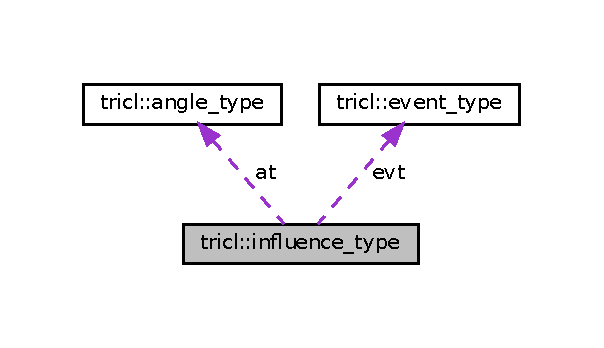
\includegraphics[width=270pt]{d0/dba/structtricl_1_1influence__type__coll__graph}
\end{center}
\end{figure}
\subsection*{Data Fields}
\begin{DoxyCompactItemize}
\item 
\mbox{\Hypertarget{structtricl_1_1influence__type_a9e3a80224b266e0ff8041644e372fe19}\label{structtricl_1_1influence__type_a9e3a80224b266e0ff8041644e372fe19}} 
const \hyperlink{structtricl_1_1event__type}{event\+\_\+type} {\bfseries evt}
\item 
\mbox{\Hypertarget{structtricl_1_1influence__type_a9d6fecd13fbb3e7b0686556d80b3b537}\label{structtricl_1_1influence__type_a9d6fecd13fbb3e7b0686556d80b3b537}} 
const \hyperlink{structtricl_1_1angle__type}{angle\+\_\+type} {\bfseries at}
\end{DoxyCompactItemize}
\subsection*{Friends}
\begin{DoxyCompactItemize}
\item 
\mbox{\Hypertarget{structtricl_1_1influence__type_a4f5b42686b09f580c15f8fa9f3aa296f}\label{structtricl_1_1influence__type_a4f5b42686b09f580c15f8fa9f3aa296f}} 
bool {\bfseries operator==} (const \hyperlink{structtricl_1_1influence__type}{influence\+\_\+type} \&left, const \hyperlink{structtricl_1_1influence__type}{influence\+\_\+type} \&right)
\end{DoxyCompactItemize}


The documentation for this struct was generated from the following file\+:\begin{DoxyCompactItemize}
\item 
src/\hyperlink{data__model_8h}{data\+\_\+model.\+h}\end{DoxyCompactItemize}

\hypertarget{structtricl_1_1inleg}{}\section{tricl\+:\+:inleg Struct Reference}
\label{structtricl_1_1inleg}\index{tricl\+::inleg@{tricl\+::inleg}}


An inleg represents a leg \char`\"{}incoming\char`\"{} to a target entity.  




{\ttfamily \#include $<$data\+\_\+model.\+h$>$}

\subsection*{Data Fields}
\begin{DoxyCompactItemize}
\item 
\mbox{\Hypertarget{structtricl_1_1inleg_a6bdf67f9629e590cebfa4b87d30cf4c6}\label{structtricl_1_1inleg_a6bdf67f9629e590cebfa4b87d30cf4c6}} 
\hyperlink{namespacetricl_a57273122278e8b301844e2a2e1f0742f}{entity} \hyperlink{structtricl_1_1inleg_a6bdf67f9629e590cebfa4b87d30cf4c6}{e\+\_\+source}
\begin{DoxyCompactList}\small\item\em Source entity of the leg. Plays a similar role as {\ttfamily e2} in an angle. \end{DoxyCompactList}\item 
\mbox{\Hypertarget{structtricl_1_1inleg_a5119f9bdfc64539b95279288762b39e3}\label{structtricl_1_1inleg_a5119f9bdfc64539b95279288762b39e3}} 
\hyperlink{namespacetricl_a2d01894944fb58a8fedc0912a48d13f8}{relationship\+\_\+or\+\_\+action\+\_\+type} \hyperlink{structtricl_1_1inleg_a5119f9bdfc64539b95279288762b39e3}{rat\+\_\+in}
\begin{DoxyCompactList}\small\item\em Plays a similar role as {\ttfamily rat23} in an angle. \end{DoxyCompactList}\end{DoxyCompactItemize}
\subsection*{Friends}
\begin{DoxyCompactItemize}
\item 
\mbox{\Hypertarget{structtricl_1_1inleg_a2882c00597e94a9fb19cde857cfe5003}\label{structtricl_1_1inleg_a2882c00597e94a9fb19cde857cfe5003}} 
bool {\bfseries operator==} (const \hyperlink{structtricl_1_1inleg}{inleg} \&left, const \hyperlink{structtricl_1_1inleg}{inleg} \&right)
\item 
\mbox{\Hypertarget{structtricl_1_1inleg_a8ddd31813cdcbb1b7c88d51fcd01cd23}\label{structtricl_1_1inleg_a8ddd31813cdcbb1b7c88d51fcd01cd23}} 
bool {\bfseries operator$<$} (const \hyperlink{structtricl_1_1inleg}{inleg} \&left, const \hyperlink{structtricl_1_1inleg}{inleg} \&right)
\end{DoxyCompactItemize}


\subsection{Detailed Description}
An inleg represents a leg \char`\"{}incoming\char`\"{} to a target entity. 

When an inleg is used, the target entity is clear from the context, hence it is not named itself in the inleg but only the source entity and relationship or action type are stored.

Inlegs may influence the attempt rate or success probability of \char`\"{}adjacent\char`\"{} events (events with the same target entity). 

The documentation for this struct was generated from the following file\+:\begin{DoxyCompactItemize}
\item 
src/\hyperlink{data__model_8h}{data\+\_\+model.\+h}\end{DoxyCompactItemize}

\hypertarget{structtricl_1_1link}{}\section{tricl\+:\+:link Struct Reference}
\label{structtricl_1_1link}\index{tricl\+::link@{tricl\+::link}}


A link encodes either the existence of a certain relationship between two entities (or the cumulative impact of all past actions of a certain type between two entities -- not yet implemented).  




{\ttfamily \#include $<$data\+\_\+model.\+h$>$}

\subsection*{Data Fields}
\begin{DoxyCompactItemize}
\item 
\mbox{\Hypertarget{structtricl_1_1link_a94b71567d0a342c8d0bf28e4fea1dff4}\label{structtricl_1_1link_a94b71567d0a342c8d0bf28e4fea1dff4}} 
const \hyperlink{namespacetricl_a57273122278e8b301844e2a2e1f0742f}{entity} \hyperlink{structtricl_1_1link_a94b71567d0a342c8d0bf28e4fea1dff4}{e1}
\begin{DoxyCompactList}\small\item\em Source entity (or, if $<$0, source entity type of a summary event) \end{DoxyCompactList}\item 
\mbox{\Hypertarget{structtricl_1_1link_a9a21745032378ca68f88966d78814be0}\label{structtricl_1_1link_a9a21745032378ca68f88966d78814be0}} 
const \hyperlink{namespacetricl_a2d01894944fb58a8fedc0912a48d13f8}{relationship\+\_\+or\+\_\+action\+\_\+type} \hyperlink{structtricl_1_1link_a9a21745032378ca68f88966d78814be0}{rat13}
\begin{DoxyCompactList}\small\item\em Type of relationship or action represented by this link. \end{DoxyCompactList}\item 
\mbox{\Hypertarget{structtricl_1_1link_ad54f7dbfcda5fd3f98ff5db897893c87}\label{structtricl_1_1link_ad54f7dbfcda5fd3f98ff5db897893c87}} 
const \hyperlink{namespacetricl_a57273122278e8b301844e2a2e1f0742f}{entity} \hyperlink{structtricl_1_1link_ad54f7dbfcda5fd3f98ff5db897893c87}{e3}
\begin{DoxyCompactList}\small\item\em Target entity (or, if $<$0, target entity type of a summary event) \end{DoxyCompactList}\end{DoxyCompactItemize}
\subsection*{Friends}
\begin{DoxyCompactItemize}
\item 
\mbox{\Hypertarget{structtricl_1_1link_a383e61e15072ef3fe9e16102dea483e0}\label{structtricl_1_1link_a383e61e15072ef3fe9e16102dea483e0}} 
bool {\bfseries operator==} (const \hyperlink{structtricl_1_1link}{link} \&left, const \hyperlink{structtricl_1_1link}{link} \&right)
\item 
\mbox{\Hypertarget{structtricl_1_1link_af79bc13140c8180154526642748b0c33}\label{structtricl_1_1link_af79bc13140c8180154526642748b0c33}} 
bool {\bfseries operator$<$} (const \hyperlink{structtricl_1_1link}{link} \&left, const \hyperlink{structtricl_1_1link}{link} \&right)
\end{DoxyCompactItemize}


\subsection{Detailed Description}
A link encodes either the existence of a certain relationship between two entities (or the cumulative impact of all past actions of a certain type between two entities -- not yet implemented). 

The documentation for this struct was generated from the following file\+:\begin{DoxyCompactItemize}
\item 
src/\hyperlink{data__model_8h}{data\+\_\+model.\+h}\end{DoxyCompactItemize}

\hypertarget{structtricl_1_1link__type}{}\section{tricl\+:\+:link\+\_\+type Struct Reference}
\label{structtricl_1_1link__type}\index{tricl\+::link\+\_\+type@{tricl\+::link\+\_\+type}}


The type of a link is given by two entity types and a relationship or action type.  




{\ttfamily \#include $<$data\+\_\+model.\+h$>$}

\subsection*{Data Fields}
\begin{DoxyCompactItemize}
\item 
\mbox{\Hypertarget{structtricl_1_1link__type_a9cb3cda7790fc4d697f6274cf0af708c}\label{structtricl_1_1link__type_a9cb3cda7790fc4d697f6274cf0af708c}} 
const \hyperlink{namespacetricl_afd4de3aedd5e48cf955f03457386e98f}{entity\+\_\+type} \hyperlink{structtricl_1_1link__type_a9cb3cda7790fc4d697f6274cf0af708c}{et1}
\begin{DoxyCompactList}\small\item\em Type of source entity e1 occurring in this type of link. \end{DoxyCompactList}\item 
\mbox{\Hypertarget{structtricl_1_1link__type_ab567b0eff4a068b28141da69c810770d}\label{structtricl_1_1link__type_ab567b0eff4a068b28141da69c810770d}} 
const \hyperlink{namespacetricl_a2d01894944fb58a8fedc0912a48d13f8}{relationship\+\_\+or\+\_\+action\+\_\+type} \hyperlink{structtricl_1_1link__type_ab567b0eff4a068b28141da69c810770d}{rat13}
\begin{DoxyCompactList}\small\item\em Type of relationship or action represented by this type of link. \end{DoxyCompactList}\item 
\mbox{\Hypertarget{structtricl_1_1link__type_ae89141e8c4719830d32c0d7fe95a184f}\label{structtricl_1_1link__type_ae89141e8c4719830d32c0d7fe95a184f}} 
const \hyperlink{namespacetricl_afd4de3aedd5e48cf955f03457386e98f}{entity\+\_\+type} \hyperlink{structtricl_1_1link__type_ae89141e8c4719830d32c0d7fe95a184f}{et3}
\begin{DoxyCompactList}\small\item\em Type of target entity e3 occurring in this type of link. \end{DoxyCompactList}\end{DoxyCompactItemize}
\subsection*{Friends}
\begin{DoxyCompactItemize}
\item 
\mbox{\Hypertarget{structtricl_1_1link__type_ae75460e218908d70af1163248317096e}\label{structtricl_1_1link__type_ae75460e218908d70af1163248317096e}} 
bool {\bfseries operator==} (const \hyperlink{structtricl_1_1link__type}{link\+\_\+type} \&left, const \hyperlink{structtricl_1_1link__type}{link\+\_\+type} \&right)
\end{DoxyCompactItemize}


\subsection{Detailed Description}
The type of a link is given by two entity types and a relationship or action type. 

The documentation for this struct was generated from the following file\+:\begin{DoxyCompactItemize}
\item 
src/\hyperlink{data__model_8h}{data\+\_\+model.\+h}\end{DoxyCompactItemize}

\hypertarget{structtricl_1_1outleg}{}\section{tricl\+:\+:outleg Struct Reference}
\label{structtricl_1_1outleg}\index{tricl\+::outleg@{tricl\+::outleg}}


An outleg represents a leg \char`\"{}outgoing\char`\"{} from a source entity.  




{\ttfamily \#include $<$data\+\_\+model.\+h$>$}

\subsection*{Data Fields}
\begin{DoxyCompactItemize}
\item 
\mbox{\Hypertarget{structtricl_1_1outleg_a126702ea981b412b0536b34457e92f45}\label{structtricl_1_1outleg_a126702ea981b412b0536b34457e92f45}} 
\hyperlink{namespacetricl_a2d01894944fb58a8fedc0912a48d13f8}{relationship\+\_\+or\+\_\+action\+\_\+type} \hyperlink{structtricl_1_1outleg_a126702ea981b412b0536b34457e92f45}{rat\+\_\+out}
\begin{DoxyCompactList}\small\item\em Plays a similar role as {\ttfamily rat12} in an angle. \end{DoxyCompactList}\item 
\mbox{\Hypertarget{structtricl_1_1outleg_a7329dd10bd2213695049e0b816ab34ce}\label{structtricl_1_1outleg_a7329dd10bd2213695049e0b816ab34ce}} 
\hyperlink{namespacetricl_a57273122278e8b301844e2a2e1f0742f}{entity} \hyperlink{structtricl_1_1outleg_a7329dd10bd2213695049e0b816ab34ce}{e\+\_\+target}
\begin{DoxyCompactList}\small\item\em Target entity of the leg. Plays a similar role as {\ttfamily e2} in an angle. \end{DoxyCompactList}\end{DoxyCompactItemize}
\subsection*{Friends}
\begin{DoxyCompactItemize}
\item 
\mbox{\Hypertarget{structtricl_1_1outleg_a925572d2a4bc56d312134f995f7790a5}\label{structtricl_1_1outleg_a925572d2a4bc56d312134f995f7790a5}} 
bool {\bfseries operator==} (const \hyperlink{structtricl_1_1outleg}{outleg} \&left, const \hyperlink{structtricl_1_1outleg}{outleg} \&right)
\item 
\mbox{\Hypertarget{structtricl_1_1outleg_a594b6be76b1271da95305f64d3f28f52}\label{structtricl_1_1outleg_a594b6be76b1271da95305f64d3f28f52}} 
bool {\bfseries operator$<$} (const \hyperlink{structtricl_1_1outleg}{outleg} \&left, const \hyperlink{structtricl_1_1outleg}{outleg} \&right)
\end{DoxyCompactItemize}


\subsection{Detailed Description}
An outleg represents a leg \char`\"{}outgoing\char`\"{} from a source entity. 

When an outleg is used, the source entity is clear from the context, hence it is not named itself in the outleg but only the target entity and relationship or action type are stored.

Outlegs may influence the attempt rate or success probability of \char`\"{}adjacent\char`\"{} events (events with the same source entity). 

The documentation for this struct was generated from the following file\+:\begin{DoxyCompactItemize}
\item 
src/\hyperlink{data__model_8h}{data\+\_\+model.\+h}\end{DoxyCompactItemize}

\chapter{File Documentation}
\hypertarget{angle_8cpp}{}\section{src/angle.cpp File Reference}
\label{angle_8cpp}\index{src/angle.\+cpp@{src/angle.\+cpp}}


Handling of angles.  


{\ttfamily \#include \char`\"{}global\+\_\+variables.\+h\char`\"{}}\newline
{\ttfamily \#include \char`\"{}probability.\+h\char`\"{}}\newline
{\ttfamily \#include \char`\"{}debugging.\+h\char`\"{}}\newline
{\ttfamily \#include \char`\"{}event.\+h\char`\"{}}\newline
{\ttfamily \#include \char`\"{}io.\+h\char`\"{}}\newline
{\ttfamily \#include \char`\"{}angle.\+h\char`\"{}}\newline
Include dependency graph for angle.\+cpp\+:
\nopagebreak
\begin{figure}[H]
\begin{center}
\leavevmode
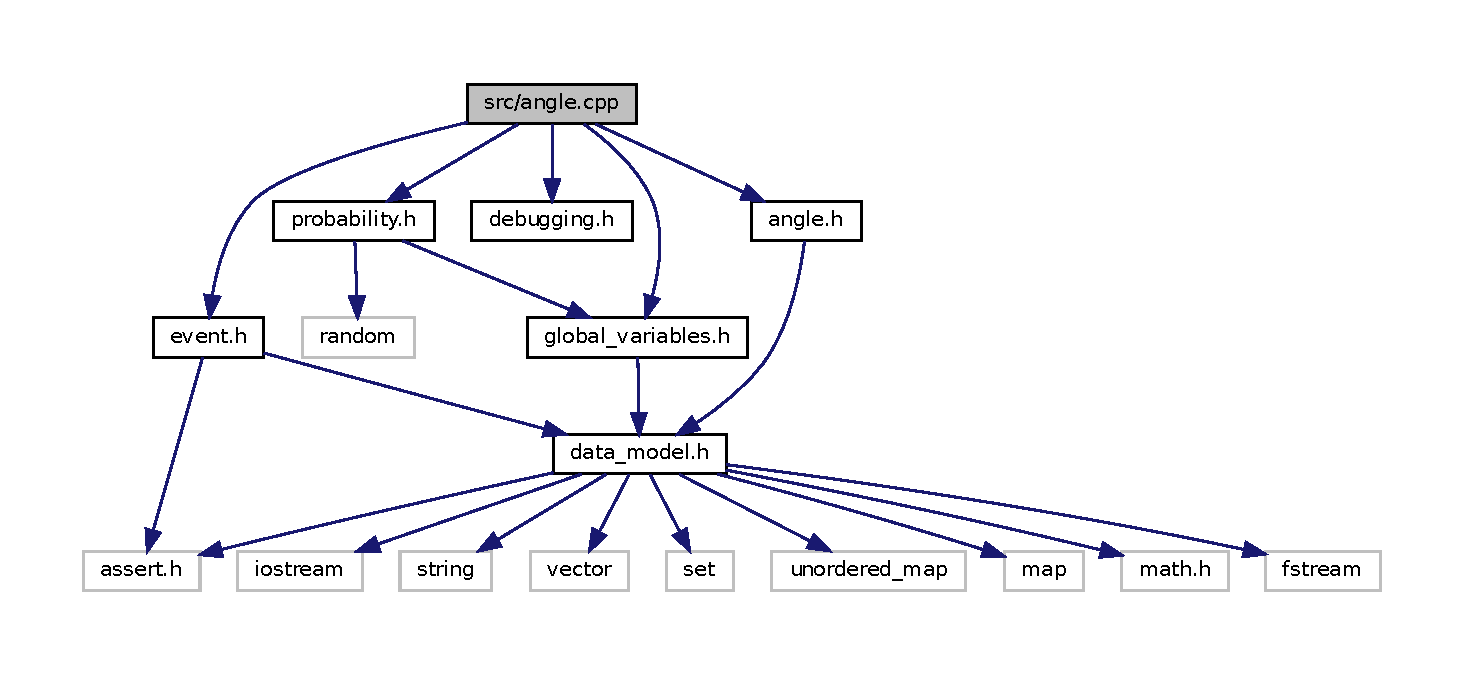
\includegraphics[width=350pt]{db/d2d/angle_8cpp__incl}
\end{center}
\end{figure}
\subsection*{Functions}
\begin{DoxyCompactItemize}
\item 
void \hyperlink{angle_8cpp_a1a5dff9417edeae00cf8bfd75459fc36}{add\+\_\+or\+\_\+delete\+\_\+angle} (\hyperlink{namespacetricl_a6967089e2c0837f273d8cb5fd9f7e46d}{event\+\_\+class} ec\+\_\+angle, \hyperlink{namespacetricl_a57273122278e8b301844e2a2e1f0742f}{entity} e1, \hyperlink{namespacetricl_afd4de3aedd5e48cf955f03457386e98f}{entity\+\_\+type} et1, \hyperlink{namespacetricl_a2d01894944fb58a8fedc0912a48d13f8}{relationship\+\_\+or\+\_\+action\+\_\+type} rat12, \hyperlink{namespacetricl_a57273122278e8b301844e2a2e1f0742f}{entity} e2, \hyperlink{namespacetricl_afd4de3aedd5e48cf955f03457386e98f}{entity\+\_\+type} et2, \hyperlink{namespacetricl_a2d01894944fb58a8fedc0912a48d13f8}{relationship\+\_\+or\+\_\+action\+\_\+type} rat23, \hyperlink{namespacetricl_a57273122278e8b301844e2a2e1f0742f}{entity} e3, \hyperlink{namespacetricl_afd4de3aedd5e48cf955f03457386e98f}{entity\+\_\+type} et3)
\begin{DoxyCompactList}\small\item\em Perform all necessary changes in state and event data due to the addition or deletion of an angle. \end{DoxyCompactList}\item 
angles \hyperlink{angle_8cpp_a866a945b4a5609c25d73c6488041a658}{leg\+\_\+intersection} (\hyperlink{namespacetricl_a57273122278e8b301844e2a2e1f0742f}{entity} e1, \hyperlink{namespacetricl_ac36fc4606da3d7f9ffd1764942fe5940}{outleg\+\_\+set} \&out1, \hyperlink{namespacetricl_a703ed53fa2dba74d8f51ede5fd46038d}{inleg\+\_\+set} \&in3, \hyperlink{namespacetricl_a57273122278e8b301844e2a2e1f0742f}{entity} e3)
\begin{DoxyCompactList}\small\item\em Compare each outleg of e1 with each inleg of e3 to find each angle from e1 to e3. \end{DoxyCompactList}\end{DoxyCompactItemize}


\subsection{Detailed Description}
Handling of angles. 

See \hyperlink{data__model_8h}{data\+\_\+model.\+h} for how a \hyperlink{structtricl_1_1angle}{tricl\+::angle} relates to other tricl datatypes. 

\subsection{Function Documentation}
\mbox{\Hypertarget{angle_8cpp_a1a5dff9417edeae00cf8bfd75459fc36}\label{angle_8cpp_a1a5dff9417edeae00cf8bfd75459fc36}} 
\index{angle.\+cpp@{angle.\+cpp}!add\+\_\+or\+\_\+delete\+\_\+angle@{add\+\_\+or\+\_\+delete\+\_\+angle}}
\index{add\+\_\+or\+\_\+delete\+\_\+angle@{add\+\_\+or\+\_\+delete\+\_\+angle}!angle.\+cpp@{angle.\+cpp}}
\subsubsection{\texorpdfstring{add\+\_\+or\+\_\+delete\+\_\+angle()}{add\_or\_delete\_angle()}}
{\footnotesize\ttfamily void add\+\_\+or\+\_\+delete\+\_\+angle (\begin{DoxyParamCaption}\item[{\hyperlink{namespacetricl_a6967089e2c0837f273d8cb5fd9f7e46d}{event\+\_\+class}}]{ec\+\_\+angle,  }\item[{\hyperlink{namespacetricl_a57273122278e8b301844e2a2e1f0742f}{entity}}]{e1,  }\item[{\hyperlink{namespacetricl_afd4de3aedd5e48cf955f03457386e98f}{entity\+\_\+type}}]{et1,  }\item[{\hyperlink{namespacetricl_a2d01894944fb58a8fedc0912a48d13f8}{relationship\+\_\+or\+\_\+action\+\_\+type}}]{rat12,  }\item[{\hyperlink{namespacetricl_a57273122278e8b301844e2a2e1f0742f}{entity}}]{e2,  }\item[{\hyperlink{namespacetricl_afd4de3aedd5e48cf955f03457386e98f}{entity\+\_\+type}}]{et2,  }\item[{\hyperlink{namespacetricl_a2d01894944fb58a8fedc0912a48d13f8}{relationship\+\_\+or\+\_\+action\+\_\+type}}]{rat23,  }\item[{\hyperlink{namespacetricl_a57273122278e8b301844e2a2e1f0742f}{entity}}]{e3,  }\item[{\hyperlink{namespacetricl_afd4de3aedd5e48cf955f03457386e98f}{entity\+\_\+type}}]{et3 }\end{DoxyParamCaption})}



Perform all necessary changes in state and event data due to the addition or deletion of an angle. 

Iterate through all events that might be influenced by this angle, update their attempt rates and success probability units, and (re)schedule them based on the new rates.

This is one of the performance bottleneck functions since it is called many times by update\+\_\+adjacent\+\_\+events(). 
\begin{DoxyParams}[1]{Parameters}
\mbox{\tt in}  & {\em ec\+\_\+angle} & class of the event that caused the change\+: E\+C\+\_\+\+E\+ST adds an angle, E\+C\+\_\+\+T\+E\+RM deletes one \\
\hline
\mbox{\tt in}  & {\em e1} & source entity \\
\hline
\mbox{\tt in}  & {\em et1} & its type \\
\hline
\mbox{\tt in}  & {\em rat12} & source-\/to-\/middle relationship or action type \\
\hline
\mbox{\tt in}  & {\em e2} & middle entity \\
\hline
\mbox{\tt in}  & {\em et2} & its type \\
\hline
\mbox{\tt in}  & {\em rat23} & middle-\/to-\/target relationship or action type \\
\hline
\mbox{\tt in}  & {\em e3} & target entity \\
\hline
\mbox{\tt in}  & {\em et3} & its type \\
\hline
\end{DoxyParams}
\mbox{\Hypertarget{angle_8cpp_a866a945b4a5609c25d73c6488041a658}\label{angle_8cpp_a866a945b4a5609c25d73c6488041a658}} 
\index{angle.\+cpp@{angle.\+cpp}!leg\+\_\+intersection@{leg\+\_\+intersection}}
\index{leg\+\_\+intersection@{leg\+\_\+intersection}!angle.\+cpp@{angle.\+cpp}}
\subsubsection{\texorpdfstring{leg\+\_\+intersection()}{leg\_intersection()}}
{\footnotesize\ttfamily angles leg\+\_\+intersection (\begin{DoxyParamCaption}\item[{\hyperlink{namespacetricl_a57273122278e8b301844e2a2e1f0742f}{entity}}]{e1,  }\item[{\hyperlink{namespacetricl_ac36fc4606da3d7f9ffd1764942fe5940}{outleg\+\_\+set} \&}]{out1,  }\item[{\hyperlink{namespacetricl_a703ed53fa2dba74d8f51ede5fd46038d}{inleg\+\_\+set} \&}]{in3,  }\item[{\hyperlink{namespacetricl_a57273122278e8b301844e2a2e1f0742f}{entity}}]{e3 }\end{DoxyParamCaption})}



Compare each outleg of e1 with each inleg of e3 to find each angle from e1 to e3. 

This is one of the performance bottleneck functions since it is called by \hyperlink{angle_8cpp_a1a5dff9417edeae00cf8bfd75459fc36}{add\+\_\+or\+\_\+delete\+\_\+angle()}.

(code was adapted from adapted from set\+\_\+intersection template)

\begin{DoxyReturn}{Returns}
a vector of found angles 
\end{DoxyReturn}
\subsubsection*{Algorithm\+: }

The two sequences are sorted by e2 (since std\+::set is an ordered datatype and operator$<$ for legs was implemented accordingly). Pseudocode\+: \begin{DoxyVerb}put blockstart = out1.end().
repeat:
  if out1.e2 < in3.e2, advance out1.
  else if out1.e2 > in3.e2:
    advance in3.
    if blockstart != out1.end():
      if in3.e2 == previous in3.e2, rewind out2 to blockstart
      else put blockstart = out1.end().
  else out1.e2 == in3.e2:
    if blockstart == out1.end(), remember out1 position as blockstart
    store found angle
    advance out1
\end{DoxyVerb}

\begin{DoxyParams}[1]{Parameters}
\mbox{\tt in}  & {\em e1} & source entity \\
\hline
\mbox{\tt in}  & {\em out1} & set of outlegs of source entity \\
\hline
\mbox{\tt in}  & {\em in3} & set of inlegs of target entity \\
\hline
\mbox{\tt in}  & {\em e3} & target entity \\
\hline
\end{DoxyParams}

\hypertarget{config_8cpp}{}\section{src/config.cpp File Reference}
\label{config_8cpp}\index{src/config.\+cpp@{src/config.\+cpp}}


Handling of configuration files.  


{\ttfamily \#include $<$limits.\+h$>$}\\*
{\ttfamily \#include $<$math.\+h$>$}\\*
{\ttfamily \#include $<$iostream$>$}\\*
{\ttfamily \#include \char`\"{}yaml-\/cpp/yaml.\+h\char`\"{}}\\*
{\ttfamily \#include \char`\"{}data\+\_\+model.\+h\char`\"{}}\\*
{\ttfamily \#include \char`\"{}global\+\_\+variables.\+h\char`\"{}}\\*
{\ttfamily \#include \char`\"{}entity.\+h\char`\"{}}\\*
{\ttfamily \#include \char`\"{}io.\+h\char`\"{}}\\*
Include dependency graph for config.\+cpp\+:
\nopagebreak
\begin{figure}[H]
\begin{center}
\leavevmode
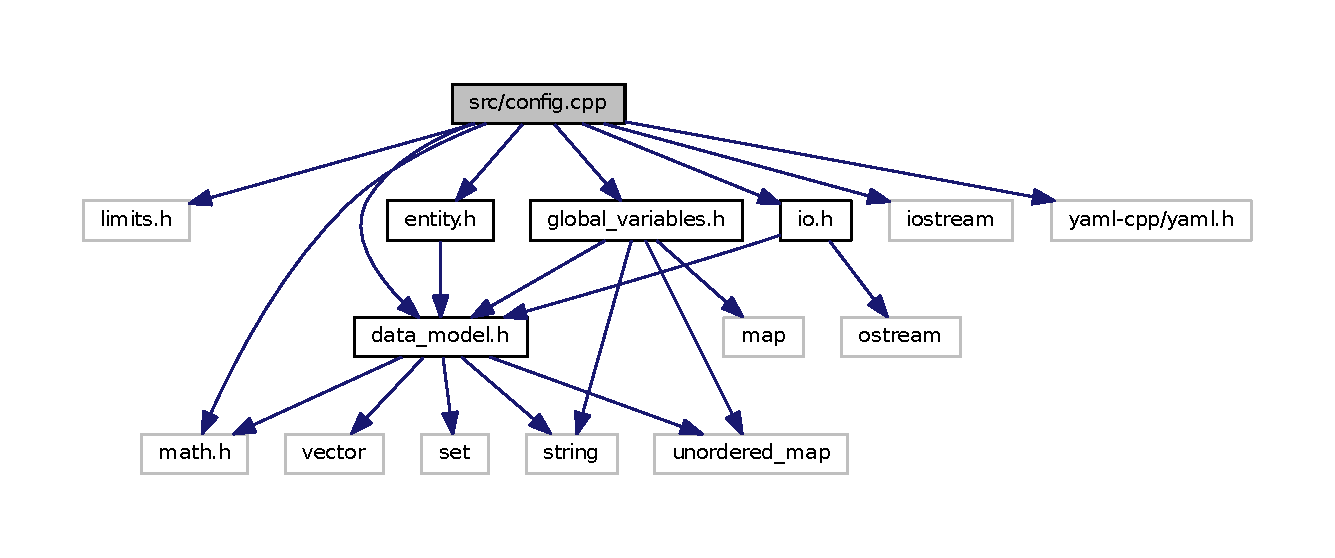
\includegraphics[width=350pt]{db/d4c/config_8cpp__incl}
\end{center}
\end{figure}
\subsection*{Macros}
\begin{DoxyCompactItemize}
\item 
\#define {\bfseries T\+A\+I\+L\+\_\+\+D\+E\+F\+A\+U\+LT}~1.\+0\hypertarget{config_8cpp_a04e254fb2bac4b90010f68d6d716f448}{}\label{config_8cpp_a04e254fb2bac4b90010f68d6d716f448}

\end{DoxyCompactItemize}
\subsection*{Functions}
\begin{DoxyCompactItemize}
\item 
void {\bfseries read\+\_\+entity\+\_\+labels} (Y\+A\+M\+L\+::\+Node n, entity\+\_\+type et)\hypertarget{config_8cpp_ac5594ed0754d45494f17470961e83309}{}\label{config_8cpp_ac5594ed0754d45494f17470961e83309}

\item 
void {\bfseries read\+\_\+config} ()\hypertarget{config_8cpp_ac8471a77a592a1fbe4b3af45fa93098a}{}\label{config_8cpp_ac8471a77a592a1fbe4b3af45fa93098a}

\end{DoxyCompactItemize}
\subsection*{Variables}
\begin{DoxyCompactItemize}
\item 
string {\bfseries gexf\+\_\+filename} = \char`\"{}\char`\"{}\hypertarget{config_8cpp_a0b60e3ce1fbd529d7fb44c1a3b6f2d5a}{}\label{config_8cpp_a0b60e3ce1fbd529d7fb44c1a3b6f2d5a}

\item 
string {\bfseries diagram\+\_\+fileprefix} = \char`\"{}\char`\"{}\hypertarget{config_8cpp_af960657d113135c47b4e0ed4536930c0}{}\label{config_8cpp_af960657d113135c47b4e0ed4536930c0}

\item 
bool {\bfseries verbose} = false\hypertarget{config_8cpp_ab3f078684998b83967d507d0f453f454}{}\label{config_8cpp_ab3f078684998b83967d507d0f453f454}

\item 
bool {\bfseries quiet} = false\hypertarget{config_8cpp_ae4426f467d61ae456b95844d4d9c2dcd}{}\label{config_8cpp_ae4426f467d61ae456b95844d4d9c2dcd}

\item 
bool {\bfseries debug} = false\hypertarget{config_8cpp_a398527b3e9e358c345c5047b16871957}{}\label{config_8cpp_a398527b3e9e358c345c5047b16871957}

\item 
timepoint {\bfseries max\+\_\+t} = I\+N\+F\+I\+N\+I\+TY\hypertarget{config_8cpp_a61e4a08c5309d5cd9538ce9654bdb9e9}{}\label{config_8cpp_a61e4a08c5309d5cd9538ce9654bdb9e9}

\item 
long int {\bfseries max\+\_\+n\+\_\+events} = L\+O\+N\+G\+\_\+\+M\+AX\hypertarget{config_8cpp_a921a3c48e5eda75a9944e3d8fdecc826}{}\label{config_8cpp_a921a3c48e5eda75a9944e3d8fdecc826}

\item 
unsigned {\bfseries seed} = 0\hypertarget{config_8cpp_abb3c5a016eb55b340002c5da33a16714}{}\label{config_8cpp_abb3c5a016eb55b340002c5da33a16714}

\item 
unordered\+\_\+map$<$ entity\+\_\+type, label $>$ {\bfseries et2label} = \{\}\hypertarget{config_8cpp_a1b14b11720f5396f884aba602cc42602}{}\label{config_8cpp_a1b14b11720f5396f884aba602cc42602}

\item 
unordered\+\_\+map$<$ string, entity\+\_\+type $>$ {\bfseries label2et} = \{\}\hypertarget{config_8cpp_a4ad1375a3f0b5760ef4861ef35ac7f25}{}\label{config_8cpp_a4ad1375a3f0b5760ef4861ef35ac7f25}

\item 
unordered\+\_\+map$<$ entity\+\_\+type, entity $>$ {\bfseries et2n} = \{\}\hypertarget{config_8cpp_aba5a0104caf66faf04d0e2f4491415fb}{}\label{config_8cpp_aba5a0104caf66faf04d0e2f4491415fb}

\item 
unordered\+\_\+map$<$ relationship\+\_\+or\+\_\+action\+\_\+type, label $>$ {\bfseries rat2label} = \{ \{R\+T\+\_\+\+ID, \char`\"{}=\char`\"{}\} \}\hypertarget{config_8cpp_a16775be180de048f5d158cf6c18af175}{}\label{config_8cpp_a16775be180de048f5d158cf6c18af175}

\item 
unordered\+\_\+map$<$ string, relationship\+\_\+or\+\_\+action\+\_\+type $>$ {\bfseries label2rat} = \{ \{\char`\"{}=\char`\"{}, R\+T\+\_\+\+ID\} \}\hypertarget{config_8cpp_a1b29491c10222b82a8ac3f8241aa27a8}{}\label{config_8cpp_a1b29491c10222b82a8ac3f8241aa27a8}

\item 
unordered\+\_\+map$<$ relationship\+\_\+or\+\_\+action\+\_\+type, bool $>$ {\bfseries r\+\_\+is\+\_\+action\+\_\+type} = \{\}\hypertarget{config_8cpp_acb03df27c0aec975d0d0a27e21f9b956}{}\label{config_8cpp_acb03df27c0aec975d0d0a27e21f9b956}

\item 
unordered\+\_\+map$<$ relationship\+\_\+or\+\_\+action\+\_\+type, relationship\+\_\+or\+\_\+action\+\_\+type $>$ {\bfseries rat2inv} = \{\}\hypertarget{config_8cpp_a698aaa515390777326d52ab118c9f1fe}{}\label{config_8cpp_a698aaa515390777326d52ab118c9f1fe}

\item 
unordered\+\_\+map$<$ entity, entity\+\_\+type $>$ {\bfseries e2et} = \{\}\hypertarget{config_8cpp_a12b15805ec2a70ba1781f87af3d8215b}{}\label{config_8cpp_a12b15805ec2a70ba1781f87af3d8215b}

\item 
unordered\+\_\+map$<$ entity, label $>$ {\bfseries e2label} = \{\}\hypertarget{config_8cpp_a1d4d2e1edc14bccb896b5dd715cba4a6}{}\label{config_8cpp_a1d4d2e1edc14bccb896b5dd715cba4a6}

\item 
unordered\+\_\+map$<$ string, entity $>$ {\bfseries label2e} = \{\}\hypertarget{config_8cpp_a3e3cf64afa14be51e4752ebe0e78d8b4}{}\label{config_8cpp_a3e3cf64afa14be51e4752ebe0e78d8b4}

\item 
set$<$ \hyperlink{structlink}{link} $>$ {\bfseries initial\+\_\+links} = \{\}\hypertarget{config_8cpp_afe42a9a97fc8e959183c94fc333f2331}{}\label{config_8cpp_afe42a9a97fc8e959183c94fc333f2331}

\item 
unordered\+\_\+map$<$ entity\+\_\+type, int $>$ {\bfseries et2n\+\_\+blocks} = \{\}\hypertarget{config_8cpp_ac3d91d4eef87cfaf1371a698513533ba}{}\label{config_8cpp_ac3d91d4eef87cfaf1371a698513533ba}

\item 
unordered\+\_\+map$<$ \hyperlink{structlink__type}{link\+\_\+type}, probability $>$ {\bfseries lt2initial\+\_\+prob\+\_\+within} = \{\}\hypertarget{config_8cpp_a1cf9b4c5338052d0ac84135ecefc7d39}{}\label{config_8cpp_a1cf9b4c5338052d0ac84135ecefc7d39}

\item 
unordered\+\_\+map$<$ \hyperlink{structlink__type}{link\+\_\+type}, probability $>$ {\bfseries lt2initial\+\_\+prob\+\_\+between} = \{\}\hypertarget{config_8cpp_aa892b7f705910915c42a59b564850a4a}{}\label{config_8cpp_aa892b7f705910915c42a59b564850a4a}

\item 
unordered\+\_\+map$<$ entity\+\_\+type, int $>$ {\bfseries et2dim} = \{\}\hypertarget{config_8cpp_a5022e1a1414fd07a51e1e3e6f08ab064}{}\label{config_8cpp_a5022e1a1414fd07a51e1e3e6f08ab064}

\item 
unordered\+\_\+map$<$ \hyperlink{structlink__type}{link\+\_\+type}, probability $>$ {\bfseries lt2spatial\+\_\+decay} = \{\}\hypertarget{config_8cpp_ac075689bc4d37b273487fa22e5099b32}{}\label{config_8cpp_ac075689bc4d37b273487fa22e5099b32}

\item 
unordered\+\_\+map$<$ \hyperlink{structinfluence__type}{influence\+\_\+type}, rate $>$ {\bfseries inflt2attempt\+\_\+rate} = \{\}\hypertarget{config_8cpp_aa37926f8d74a0c74e47def544c4f872e}{}\label{config_8cpp_aa37926f8d74a0c74e47def544c4f872e}

\item 
unordered\+\_\+map$<$ \hyperlink{structevent__type}{event\+\_\+type}, double $>$ {\bfseries evt2left\+\_\+tail} = \{\}\hypertarget{config_8cpp_ae7b89a8070b4de9d132b167704229c70}{}\label{config_8cpp_ae7b89a8070b4de9d132b167704229c70}

\item 
unordered\+\_\+map$<$ \hyperlink{structevent__type}{event\+\_\+type}, double $>$ {\bfseries evt2right\+\_\+tail} = \{\}\hypertarget{config_8cpp_a6a65e62a5f8173784beb092165af2528}{}\label{config_8cpp_a6a65e62a5f8173784beb092165af2528}

\item 
unordered\+\_\+map$<$ \hyperlink{structevent__type}{event\+\_\+type}, probunits $>$ {\bfseries evt2base\+\_\+probunits} = \{\}\hypertarget{config_8cpp_a5372b5c53ebbceff39a367177d0e4c38}{}\label{config_8cpp_a5372b5c53ebbceff39a367177d0e4c38}

\item 
unordered\+\_\+map$<$ \hyperlink{structinfluence__type}{influence\+\_\+type}, probunits $>$ {\bfseries inflt2delta\+\_\+probunits} = \{\}\hypertarget{config_8cpp_aa4d1d1a030f8a8b177f11e3b4dc93011}{}\label{config_8cpp_aa4d1d1a030f8a8b177f11e3b4dc93011}

\item 
unordered\+\_\+map$<$ entity\+\_\+type, double $>$ {\bfseries et2gexf\+\_\+size} = \{\}\hypertarget{config_8cpp_a922d0c80d1e0778e68aaca86945eb49e}{}\label{config_8cpp_a922d0c80d1e0778e68aaca86945eb49e}

\item 
unordered\+\_\+map$<$ entity\+\_\+type, double $>$ {\bfseries et2gexf\+\_\+a} = \{\}\hypertarget{config_8cpp_a26668024dfdce9d505c1e0ed03a645a2}{}\label{config_8cpp_a26668024dfdce9d505c1e0ed03a645a2}

\item 
unordered\+\_\+map$<$ entity\+\_\+type, string $>$ {\bfseries et2gexf\+\_\+shape} = \{\}\hypertarget{config_8cpp_a10ef80ac6e92253faba86527383b0b19}{}\label{config_8cpp_a10ef80ac6e92253faba86527383b0b19}

\item 
unordered\+\_\+map$<$ entity\+\_\+type, int $>$ {\bfseries et2gexf\+\_\+r} = \{\}\hypertarget{config_8cpp_aa7267315093f6567077ec5e612b46ed1}{}\label{config_8cpp_aa7267315093f6567077ec5e612b46ed1}

\item 
unordered\+\_\+map$<$ entity\+\_\+type, int $>$ {\bfseries et2gexf\+\_\+g} = \{\}\hypertarget{config_8cpp_a86c65c01b4b0c35b56baf6d8d557d977}{}\label{config_8cpp_a86c65c01b4b0c35b56baf6d8d557d977}

\item 
unordered\+\_\+map$<$ entity\+\_\+type, int $>$ {\bfseries et2gexf\+\_\+b} = \{\}\hypertarget{config_8cpp_aded47b9a1ea0cb3ac40ea0ae60d013c3}{}\label{config_8cpp_aded47b9a1ea0cb3ac40ea0ae60d013c3}

\item 
unordered\+\_\+map$<$ relationship\+\_\+or\+\_\+action\+\_\+type, double $>$ {\bfseries rat2gexf\+\_\+thickness} = \{\}\hypertarget{config_8cpp_a7e4baebe848adb451c45c44624784a8a}{}\label{config_8cpp_a7e4baebe848adb451c45c44624784a8a}

\item 
unordered\+\_\+map$<$ relationship\+\_\+or\+\_\+action\+\_\+type, double $>$ {\bfseries rat2gexf\+\_\+a} = \{\}\hypertarget{config_8cpp_a8fc9665235760bdb38eb6a631e654077}{}\label{config_8cpp_a8fc9665235760bdb38eb6a631e654077}

\item 
unordered\+\_\+map$<$ relationship\+\_\+or\+\_\+action\+\_\+type, string $>$ {\bfseries rat2gexf\+\_\+shape} = \{\}\hypertarget{config_8cpp_a9a7b4c97b0337eec7a107d4f48c994f0}{}\label{config_8cpp_a9a7b4c97b0337eec7a107d4f48c994f0}

\item 
unordered\+\_\+map$<$ relationship\+\_\+or\+\_\+action\+\_\+type, int $>$ {\bfseries rat2gexf\+\_\+r} = \{\}\hypertarget{config_8cpp_ad77fa8d20dd7cf1471f2219765253a49}{}\label{config_8cpp_ad77fa8d20dd7cf1471f2219765253a49}

\item 
unordered\+\_\+map$<$ relationship\+\_\+or\+\_\+action\+\_\+type, int $>$ {\bfseries rat2gexf\+\_\+g} = \{\}\hypertarget{config_8cpp_a8063993d6d713ccd233e2fcc6e9bc99b}{}\label{config_8cpp_a8063993d6d713ccd233e2fcc6e9bc99b}

\item 
unordered\+\_\+map$<$ relationship\+\_\+or\+\_\+action\+\_\+type, int $>$ {\bfseries rat2gexf\+\_\+b} = \{\}\hypertarget{config_8cpp_aa91b7e25dfb65b3ea4d7f4c15a7bc25d}{}\label{config_8cpp_aa91b7e25dfb65b3ea4d7f4c15a7bc25d}

\item 
entity {\bfseries max\+\_\+e} = 0\hypertarget{config_8cpp_aca8167edc3c91cb84c829dd88f75c7b4}{}\label{config_8cpp_aca8167edc3c91cb84c829dd88f75c7b4}

\end{DoxyCompactItemize}


\subsection{Detailed Description}
Handling of configuration files. 

Configuration files are in Y\+A\+ML. See config\+\_\+files/parameters\+\_\+\+T\+E\+M\+P\+L\+A\+T\+E.\+yaml for an example

\begin{DoxyAuthor}{Author}
Jobst Heitzig, Potsdam Institute for Climate Impact Research, \href{mailto:heitzig@pik-potsdam.de}{\tt heitzig@pik-\/potsdam.\+de} 
\end{DoxyAuthor}
\begin{DoxyDate}{Date}
Mar 30, 2020 
\end{DoxyDate}

\hypertarget{constants_8cpp}{}\section{src/constants.cpp File Reference}
\label{constants_8cpp}\index{src/constants.\+cpp@{src/constants.\+cpp}}


Some global constants.  


{\ttfamily \#include \char`\"{}data\+\_\+model.\+h\char`\"{}}\newline
Include dependency graph for constants.\+cpp\+:
\nopagebreak
\begin{figure}[H]
\begin{center}
\leavevmode
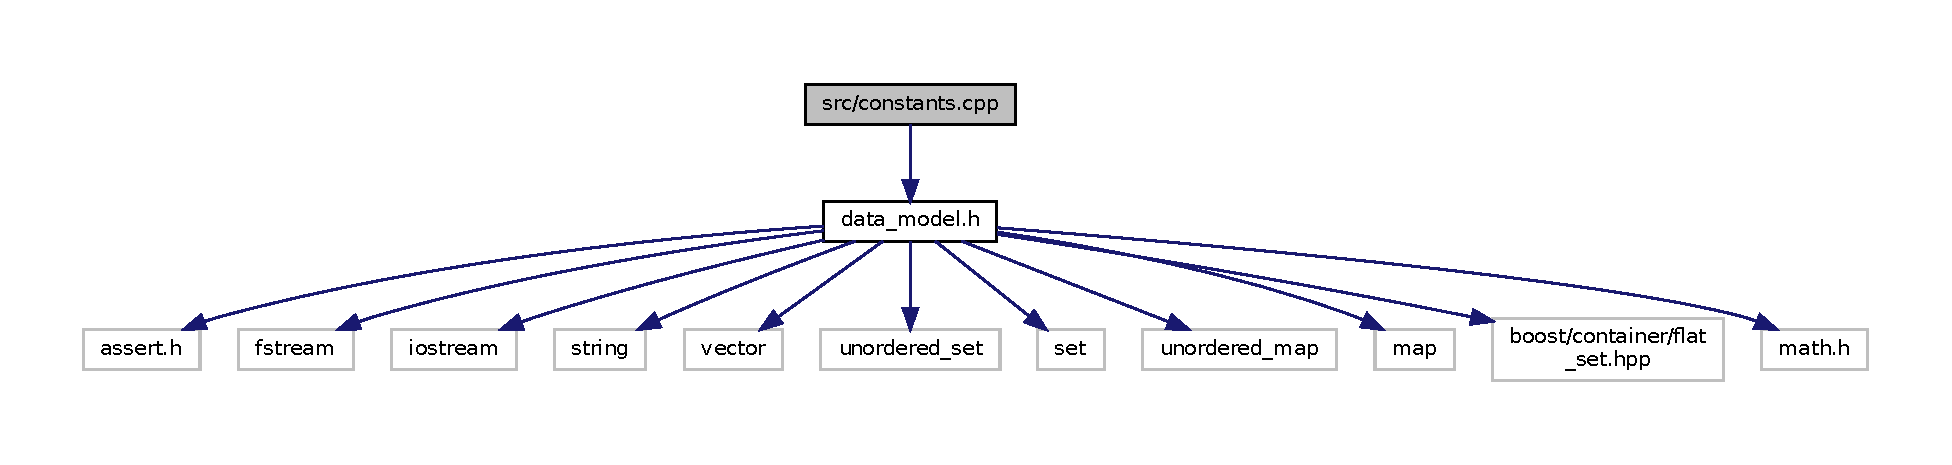
\includegraphics[width=350pt]{d0/d49/constants_8cpp__incl}
\end{center}
\end{figure}
\subsection*{Variables}
\begin{DoxyCompactItemize}
\item 
unordered\+\_\+map$<$ event\+\_\+class, string $>$ {\bfseries tricl\+::ec2label}
\end{DoxyCompactItemize}


\subsection{Detailed Description}
Some global constants. 

\begin{DoxyAuthor}{Author}
Jobst Heitzig, Potsdam Institute for Climate Impact Research, \href{mailto:heitzig@pik-potsdam.de}{\tt heitzig@pik-\/potsdam.\+de} 
\end{DoxyAuthor}
\begin{DoxyDate}{Date}
Mar 30, 2020 
\end{DoxyDate}


\subsection{Variable Documentation}
\mbox{\Hypertarget{constants_8cpp_file_a9f4cb99ed8a0723da68503403d270bf7}\label{constants_8cpp_file_a9f4cb99ed8a0723da68503403d270bf7}} 
\index{constants.\+cpp@{constants.\+cpp}!ec2label@{ec2label}}
\index{ec2label@{ec2label}!constants.\+cpp@{constants.\+cpp}}
\subsubsection{\texorpdfstring{ec2label}{ec2label}}
{\footnotesize\ttfamily unordered\+\_\+map$<$ event\+\_\+class, string $>$ tricl\+::ec2label}

{\bfseries Initial value\+:}
\begin{DoxyCode}
= \{
        \{ EC\_EST, \textcolor{stringliteral}{"establish that"} \},
        \{ EC\_TERM, \textcolor{stringliteral}{"terminate that"} \},
        \{ EC\_ACT, \textcolor{stringliteral}{"let"} \}
    \}
\end{DoxyCode}

\hypertarget{data__model_8h}{}\section{src/data\+\_\+model.h File Reference}
\label{data__model_8h}\index{src/data\+\_\+model.\+h@{src/data\+\_\+model.\+h}}


The main data model.  


{\ttfamily \#include $<$assert.\+h$>$}\newline
{\ttfamily \#include $<$fstream$>$}\newline
{\ttfamily \#include $<$iostream$>$}\newline
{\ttfamily \#include $<$string$>$}\newline
{\ttfamily \#include $<$vector$>$}\newline
{\ttfamily \#include $<$set$>$}\newline
{\ttfamily \#include $<$unordered\+\_\+map$>$}\newline
{\ttfamily \#include $<$map$>$}\newline
{\ttfamily \#include $<$math.\+h$>$}\newline
Include dependency graph for data\+\_\+model.\+h\+:\nopagebreak
\begin{figure}[H]
\begin{center}
\leavevmode
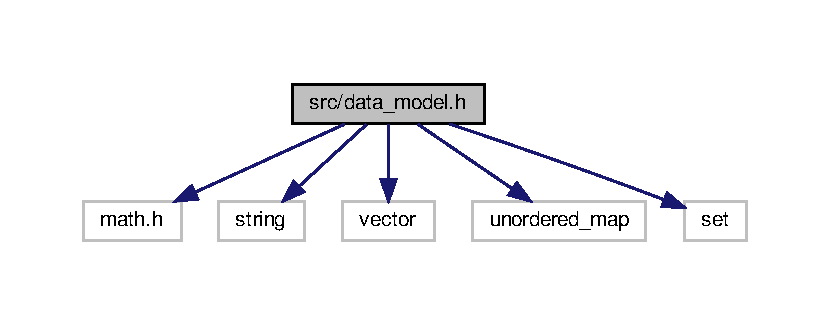
\includegraphics[width=350pt]{d0/dc6/data__model_8h__incl}
\end{center}
\end{figure}
This graph shows which files directly or indirectly include this file\+:\nopagebreak
\begin{figure}[H]
\begin{center}
\leavevmode
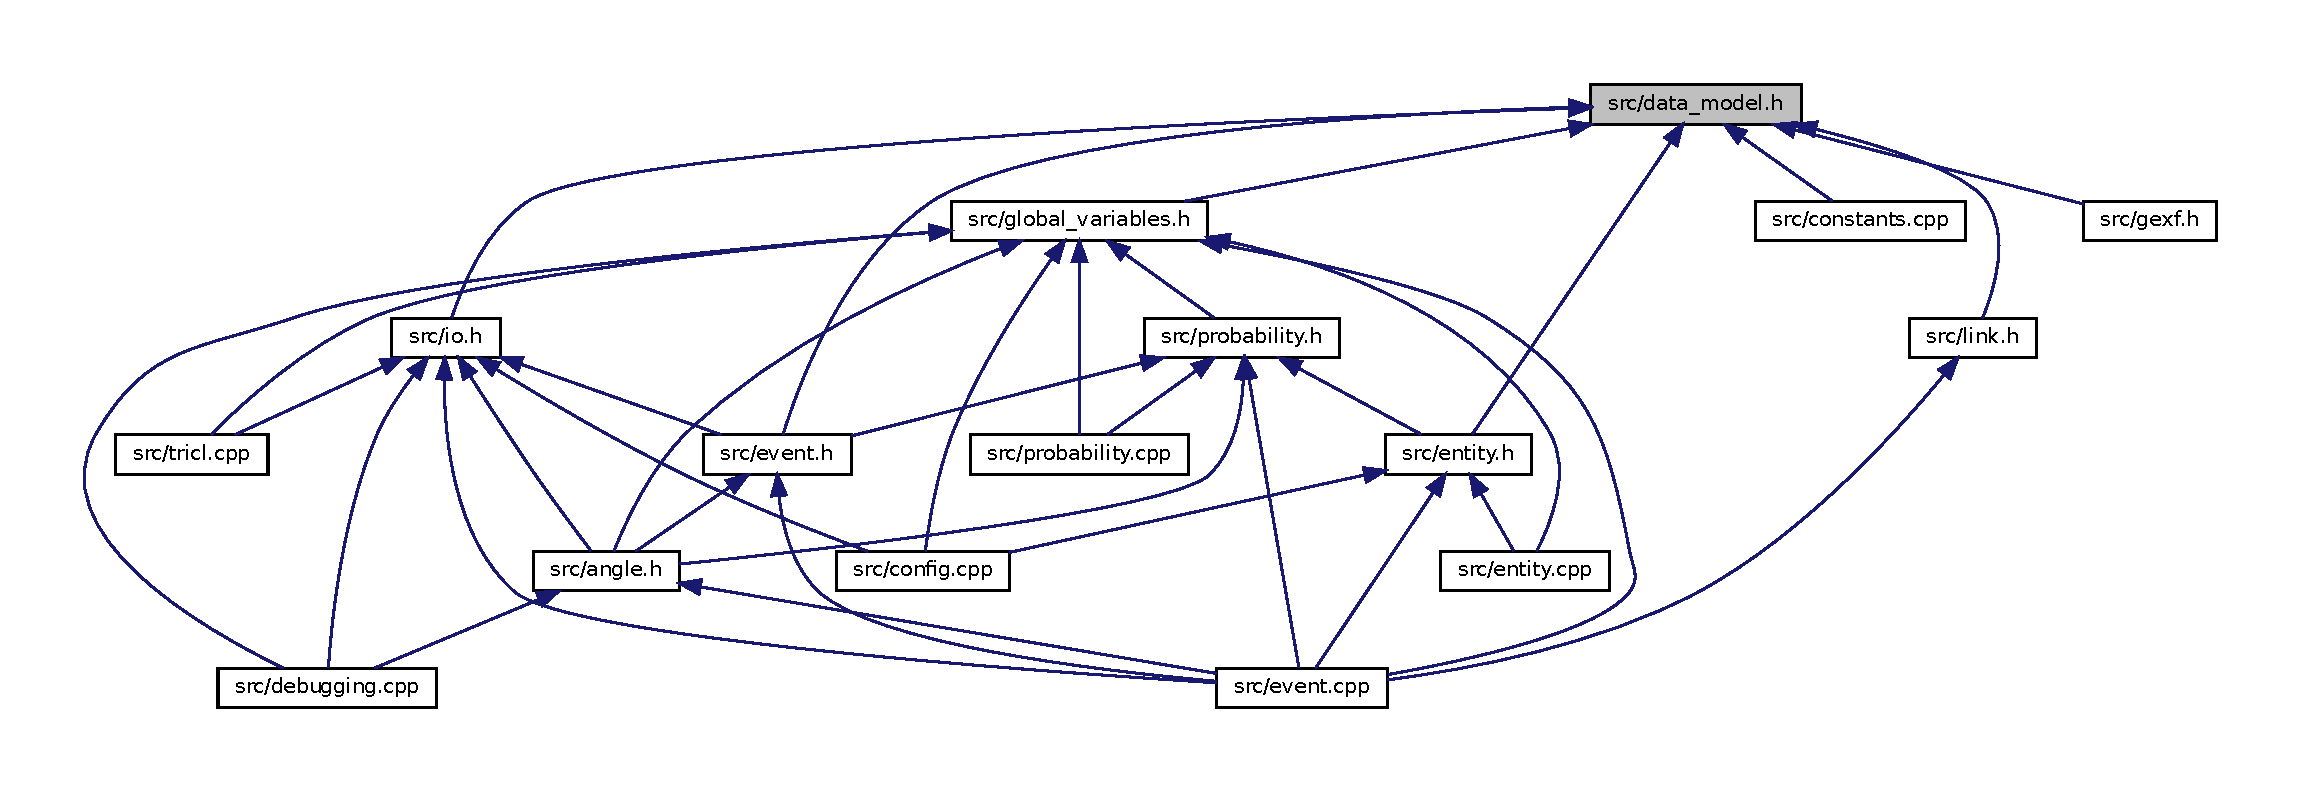
\includegraphics[width=350pt]{d8/d95/data__model_8h__dep__incl}
\end{center}
\end{figure}
\subsection*{Data Structures}
\begin{DoxyCompactItemize}
\item 
struct \hyperlink{structtricl_1_1entity__type__pair}{tricl\+::entity\+\_\+type\+\_\+pair}
\item 
struct \hyperlink{structtricl_1_1link__type}{tricl\+::link\+\_\+type}
\item 
struct \hyperlink{structtricl_1_1event__type}{tricl\+::event\+\_\+type}
\item 
struct \hyperlink{structtricl_1_1angle__type}{tricl\+::angle\+\_\+type}
\item 
struct \hyperlink{structtricl_1_1influence__type}{tricl\+::influence\+\_\+type}
\item 
struct \hyperlink{structtricl_1_1inleg}{tricl\+::inleg}
\item 
struct \hyperlink{structtricl_1_1outleg}{tricl\+::outleg}
\item 
struct \hyperlink{structtricl_1_1link}{tricl\+::link}
\item 
struct \hyperlink{structtricl_1_1event}{tricl\+::event}
\item 
struct \hyperlink{structtricl_1_1event__data}{tricl\+::event\+\_\+data}
\item 
struct \hyperlink{structtricl_1_1angle}{tricl\+::angle}
\item 
struct \hyperlink{structstd_1_1hash_3_01entity__type__pair_01_4}{std\+::hash$<$ entity\+\_\+type\+\_\+pair $>$}
\item 
struct \hyperlink{structstd_1_1hash_3_01link__type_01_4}{std\+::hash$<$ link\+\_\+type $>$}
\item 
struct \hyperlink{structstd_1_1hash_3_01event__type_01_4}{std\+::hash$<$ event\+\_\+type $>$}
\item 
struct \hyperlink{structstd_1_1hash_3_01angle__type_01_4}{std\+::hash$<$ angle\+\_\+type $>$}
\item 
struct \hyperlink{structstd_1_1hash_3_01influence__type_01_4}{std\+::hash$<$ influence\+\_\+type $>$}
\item 
struct \hyperlink{structstd_1_1hash_3_01inleg_01_4}{std\+::hash$<$ inleg $>$}
\item 
struct \hyperlink{structstd_1_1hash_3_01outleg_01_4}{std\+::hash$<$ outleg $>$}
\item 
struct \hyperlink{structstd_1_1hash_3_01link_01_4}{std\+::hash$<$ link $>$}
\item 
struct \hyperlink{structstd_1_1hash_3_01event_01_4}{std\+::hash$<$ event $>$}
\item 
struct \hyperlink{structstd_1_1hash_3_01angle_01_4}{std\+::hash$<$ angle $>$}
\end{DoxyCompactItemize}
\subsection*{Macros}
\begin{DoxyCompactItemize}
\item 
\mbox{\Hypertarget{data__model_8h_a4ef43416c3082b95dfc7b9b4b37ed4a7}\label{data__model_8h_a4ef43416c3082b95dfc7b9b4b37ed4a7}} 
\#define \hyperlink{data__model_8h_a4ef43416c3082b95dfc7b9b4b37ed4a7}{E\+\_\+\+B\+I\+TS}~20
\begin{DoxyCompactList}\small\item\em no. of bits used for entity ids --$>$ max. 1 mio. entities \end{DoxyCompactList}\item 
\mbox{\Hypertarget{data__model_8h_a27e24a1c84c197041afdad0fc49dcaeb}\label{data__model_8h_a27e24a1c84c197041afdad0fc49dcaeb}} 
\#define \hyperlink{data__model_8h_a27e24a1c84c197041afdad0fc49dcaeb}{E\+T\+\_\+\+B\+I\+TS}~4
\begin{DoxyCompactList}\small\item\em no. of bits used for entity types --$>$ max. 16 entity types \end{DoxyCompactList}\item 
\mbox{\Hypertarget{data__model_8h_a1712faaa1ef9bb3dcbfae56161881708}\label{data__model_8h_a1712faaa1ef9bb3dcbfae56161881708}} 
\#define \hyperlink{data__model_8h_a1712faaa1ef9bb3dcbfae56161881708}{R\+A\+T\+\_\+\+B\+I\+TS}~4
\begin{DoxyCompactList}\small\item\em no. of bits used for relationship or action types --$>$ max. 16 relationship or action types \end{DoxyCompactList}\item 
\mbox{\Hypertarget{data__model_8h_acaa7fd772f80b3066211e5eb6e29ed91}\label{data__model_8h_acaa7fd772f80b3066211e5eb6e29ed91}} 
\#define \hyperlink{data__model_8h_acaa7fd772f80b3066211e5eb6e29ed91}{M\+A\+X\+\_\+\+N\+\_\+E}~((1$<$$<$\hyperlink{data__model_8h_a4ef43416c3082b95dfc7b9b4b37ed4a7}{E\+\_\+\+B\+I\+TS})-\/1)
\begin{DoxyCompactList}\small\item\em resulting max. no. of entities \end{DoxyCompactList}\item 
\mbox{\Hypertarget{data__model_8h_ae71ff63a5bdb6bfc09a18840c8df4e54}\label{data__model_8h_ae71ff63a5bdb6bfc09a18840c8df4e54}} 
\#define \hyperlink{data__model_8h_ae71ff63a5bdb6bfc09a18840c8df4e54}{N\+O\+\_\+\+R\+AT}~0
\begin{DoxyCompactList}\small\item\em missing value for relationship or action type, used in angles to encode legs \end{DoxyCompactList}\item 
\mbox{\Hypertarget{data__model_8h_a549fa469b9ccb6e0fe046f797bc181e0}\label{data__model_8h_a549fa469b9ccb6e0fe046f797bc181e0}} 
\#define \hyperlink{data__model_8h_a549fa469b9ccb6e0fe046f797bc181e0}{R\+T\+\_\+\+ID}~1
\begin{DoxyCompactList}\small\item\em relationship type for identity relationship \char`\"{}=\char`\"{}, always present \end{DoxyCompactList}\item 
\mbox{\Hypertarget{data__model_8h_a9a89b5cd637aedee7c32dc74252da764}\label{data__model_8h_a9a89b5cd637aedee7c32dc74252da764}} 
\#define {\bfseries I\+N\+F\+LT}(inflt)~((size\+\_\+t)inflt.\+evt.\+ec $^\wedge$ ((size\+\_\+t)inflt.\+evt.\+et1 $<$$<$ 2) $^\wedge$ ((size\+\_\+t)inflt.\+evt.\+rat13 $<$$<$ (2+\hyperlink{data__model_8h_a27e24a1c84c197041afdad0fc49dcaeb}{E\+T\+\_\+\+B\+I\+TS})) $^\wedge$ ((size\+\_\+t)inflt.\+evt.\+et3 $<$$<$ (2+\hyperlink{data__model_8h_a27e24a1c84c197041afdad0fc49dcaeb}{E\+T\+\_\+\+B\+I\+TS}+\hyperlink{data__model_8h_a1712faaa1ef9bb3dcbfae56161881708}{R\+A\+T\+\_\+\+B\+I\+TS})) $^\wedge$ ((size\+\_\+t)inflt.\+at.\+rat12 $<$$<$ (2+2$\ast$\hyperlink{data__model_8h_a27e24a1c84c197041afdad0fc49dcaeb}{E\+T\+\_\+\+B\+I\+TS}+\hyperlink{data__model_8h_a1712faaa1ef9bb3dcbfae56161881708}{R\+A\+T\+\_\+\+B\+I\+TS})) $^\wedge$ ((size\+\_\+t)inflt.\+at.\+et2 $<$$<$ (2+2$\ast$\hyperlink{data__model_8h_a27e24a1c84c197041afdad0fc49dcaeb}{E\+T\+\_\+\+B\+I\+TS}+2$\ast$\hyperlink{data__model_8h_a1712faaa1ef9bb3dcbfae56161881708}{R\+A\+T\+\_\+\+B\+I\+TS})) $^\wedge$ ((size\+\_\+t)inflt.\+at.\+rat23 $<$$<$ (2+3$\ast$\hyperlink{data__model_8h_a27e24a1c84c197041afdad0fc49dcaeb}{E\+T\+\_\+\+B\+I\+TS}+2$\ast$\hyperlink{data__model_8h_a1712faaa1ef9bb3dcbfae56161881708}{R\+A\+T\+\_\+\+B\+I\+TS})))
\item 
\mbox{\Hypertarget{data__model_8h_a3890372a566c5b111dd6fabda11e73bc}\label{data__model_8h_a3890372a566c5b111dd6fabda11e73bc}} 
\#define {\bfseries M\+A\+X\+\_\+\+N\+\_\+\+I\+N\+F\+LT}~(1 $<$$<$ (2+3$\ast$\hyperlink{data__model_8h_a27e24a1c84c197041afdad0fc49dcaeb}{E\+T\+\_\+\+B\+I\+TS}+3$\ast$\hyperlink{data__model_8h_a1712faaa1ef9bb3dcbfae56161881708}{R\+A\+T\+\_\+\+B\+I\+TS}))
\end{DoxyCompactItemize}
\subsection*{Typedefs}
\begin{DoxyCompactItemize}
\item 
\mbox{\Hypertarget{data__model_8h_a720ff6a29f998e11e1d3622fc8df64b1}\label{data__model_8h_a720ff6a29f998e11e1d3622fc8df64b1}} 
typedef double \hyperlink{data__model_8h_a720ff6a29f998e11e1d3622fc8df64b1}{tricl\+::timepoint}
\begin{DoxyCompactList}\small\item\em a point in continuous model time, 0...inf \end{DoxyCompactList}\item 
\mbox{\Hypertarget{data__model_8h_af8f8f9076e92e1c664ffa96f18d038a5}\label{data__model_8h_af8f8f9076e92e1c664ffa96f18d038a5}} 
typedef double \hyperlink{data__model_8h_af8f8f9076e92e1c664ffa96f18d038a5}{tricl\+::probunits}
\begin{DoxyCompactList}\small\item\em -\/inf...inf, will be mapped to probabilities by means of the function probunits2probability() \end{DoxyCompactList}\item 
\mbox{\Hypertarget{data__model_8h_af2e8973ba58a3dad9061296d8bee16a2}\label{data__model_8h_af2e8973ba58a3dad9061296d8bee16a2}} 
typedef double \hyperlink{data__model_8h_af2e8973ba58a3dad9061296d8bee16a2}{tricl\+::probability}
\begin{DoxyCompactList}\small\item\em 0...1 \end{DoxyCompactList}\item 
\mbox{\Hypertarget{data__model_8h_ae42d2696f294300a43e0f5edf4875479}\label{data__model_8h_ae42d2696f294300a43e0f5edf4875479}} 
typedef double \hyperlink{data__model_8h_ae42d2696f294300a43e0f5edf4875479}{tricl\+::rate}
\begin{DoxyCompactList}\small\item\em probability per time, 0...inf. (inf is used for things happening \char`\"{}immediately\char`\"{}) \end{DoxyCompactList}\item 
\mbox{\Hypertarget{data__model_8h_a77e7daffafa870e5786b344119da9b15}\label{data__model_8h_a77e7daffafa870e5786b344119da9b15}} 
typedef string \hyperlink{data__model_8h_a77e7daffafa870e5786b344119da9b15}{tricl\+::label}
\begin{DoxyCompactList}\small\item\em labels of things \end{DoxyCompactList}\item 
typedef int \hyperlink{data__model_8h_a57273122278e8b301844e2a2e1f0742f}{tricl\+::entity}
\begin{DoxyCompactList}\small\item\em Entities are used to encode all physical and abstract objects of the modeled social dynamics that can stand in some form of relation to another or can perform some kinds of actions on or with another. \end{DoxyCompactList}\item 
typedef short unsigned int \hyperlink{data__model_8h_afd4de3aedd5e48cf955f03457386e98f}{tricl\+::entity\+\_\+type}
\begin{DoxyCompactList}\small\item\em Entity types are used to encode the different kinds of entities in a model. \end{DoxyCompactList}\item 
typedef size\+\_\+t \hyperlink{data__model_8h_a2d01894944fb58a8fedc0912a48d13f8}{tricl\+::relationship\+\_\+or\+\_\+action\+\_\+type}
\begin{DoxyCompactList}\small\item\em Relationship types are used to encode the kinds of relationships entities may stand in; action types are used to encode the kinds of actions entities may perform on or with another (not implemented yet); they are encoded in a common datatype and distinguished by means of the map rat\+\_\+is\+\_\+action\+\_\+type (not implemented yet). \end{DoxyCompactList}\item 
\mbox{\Hypertarget{data__model_8h_a703ed53fa2dba74d8f51ede5fd46038d}\label{data__model_8h_a703ed53fa2dba74d8f51ede5fd46038d}} 
typedef set$<$ \hyperlink{structtricl_1_1inleg}{inleg} $>$ {\bfseries tricl\+::inleg\+\_\+set}
\item 
\mbox{\Hypertarget{data__model_8h_ac36fc4606da3d7f9ffd1764942fe5940}\label{data__model_8h_ac36fc4606da3d7f9ffd1764942fe5940}} 
typedef set$<$ \hyperlink{structtricl_1_1outleg}{outleg} $>$ {\bfseries tricl\+::outleg\+\_\+set}
\item 
\mbox{\Hypertarget{data__model_8h_a4ec9b46d6dae5a1d114387bca4029ce5}\label{data__model_8h_a4ec9b46d6dae5a1d114387bca4029ce5}} 
typedef vector$<$ \hyperlink{structtricl_1_1angle}{angle} $>$ {\bfseries tricl\+::angles}
\end{DoxyCompactItemize}
\subsection*{Enumerations}
\begin{DoxyCompactItemize}
\item 
enum \hyperlink{data__model_8h_a6967089e2c0837f273d8cb5fd9f7e46d}{tricl\+::event\+\_\+class} \{ \hyperlink{data__model_8h_a6967089e2c0837f273d8cb5fd9f7e46da928305067790de15396de8fcc92b72b9}{tricl\+::\+E\+C\+\_\+\+E\+ST}, 
\hyperlink{data__model_8h_a6967089e2c0837f273d8cb5fd9f7e46da16f53be37a75a1cdfc726014c7f3810a}{tricl\+::\+E\+C\+\_\+\+T\+E\+RM}, 
\hyperlink{data__model_8h_a6967089e2c0837f273d8cb5fd9f7e46dac508c68c92ee059322cb644dd330bbcf}{tricl\+::\+E\+C\+\_\+\+A\+CT}
 \}\begin{DoxyCompactList}\small\item\em (don\textquotesingle{}t confuse with event\+\_\+type!) \end{DoxyCompactList}
\end{DoxyCompactItemize}
\subsection*{Variables}
\begin{DoxyCompactItemize}
\item 
\mbox{\Hypertarget{data__model_8h_a1d25690adbc3921709bd3b3e16415713}\label{data__model_8h_a1d25690adbc3921709bd3b3e16415713}} 
const \hyperlink{structtricl_1_1angle__type}{angle\+\_\+type} {\bfseries tricl\+::\+N\+O\+\_\+\+A\+N\+G\+LE} = \{ .rat12 = \hyperlink{data__model_8h_ae71ff63a5bdb6bfc09a18840c8df4e54}{N\+O\+\_\+\+R\+AT}, .et2 = 0, .rat23 = \hyperlink{data__model_8h_ae71ff63a5bdb6bfc09a18840c8df4e54}{N\+O\+\_\+\+R\+AT} \}
\end{DoxyCompactItemize}


\subsection{Detailed Description}
The main data model. 

Defines all structs and their operators.

\begin{DoxyAuthor}{Author}
Jobst Heitzig, Potsdam Institute for Climate Impact Research, \href{mailto:heitzig@pik-potsdam.de}{\tt heitzig@pik-\/potsdam.\+de} 
\end{DoxyAuthor}
\begin{DoxyDate}{Date}
Mar 30, 2020
\end{DoxyDate}
\subsubsection*{Data architecture }

Most data is kept in unordered maps (what would be dictionaries in python) whose keys are entity types, entities, link types, links, legs, angles, event types, events, influence types and influences. the latter types of things are encoded as structs, most of which are basically tuples of integer ids.

For fast access to map entries, these are automatically turned into integer hashs via the hash structs at the end of this file.

Some data (which is accessed most often) is instead kept in vectors whose indices are either entities (which are ints) or integer hash values of influence types (constructed via the macro I\+N\+F\+LT).

All hashs are constructed as logical O\+Rs of properly shifted ids, hence valid ids are restricted by the respective numbers of bits reserved for this id in the hash.

This hash construction is governed by the bit size macros \hyperlink{data__model_8h_a4ef43416c3082b95dfc7b9b4b37ed4a7}{E\+\_\+\+B\+I\+TS}, \hyperlink{data__model_8h_a27e24a1c84c197041afdad0fc49dcaeb}{E\+T\+\_\+\+B\+I\+TS}, and \hyperlink{data__model_8h_a1712faaa1ef9bb3dcbfae56161881708}{R\+A\+T\+\_\+\+B\+I\+TS}, which could be adapted in dependence on system architecture, but must fulfil the following constraints\+: 2 + 2$\ast$\+E\+\_\+\+B\+I\+TS + R\+A\+T\+\_\+\+B\+I\+TS $<$= no. of bits in size\+\_\+t (32 or 64) 2$^\wedge$\+E\+\_\+\+B\+I\+TS + 2$^\wedge$(6 + 3$\ast$\+R\+A\+T\+\_\+\+B\+I\+TS + 3$\ast$\+E\+T\+\_\+\+B\+I\+TS) $<$= available memory bytes 

\subsection{Typedef Documentation}
\mbox{\Hypertarget{data__model_8h_file_a57273122278e8b301844e2a2e1f0742f}\label{data__model_8h_file_a57273122278e8b301844e2a2e1f0742f}} 
\index{data\+\_\+model.\+h@{data\+\_\+model.\+h}!entity@{entity}}
\index{entity@{entity}!data\+\_\+model.\+h@{data\+\_\+model.\+h}}
\subsubsection{\texorpdfstring{entity}{entity}}
{\footnotesize\ttfamily typedef int \hyperlink{data__model_8h_a57273122278e8b301844e2a2e1f0742f}{tricl\+::entity}}



Entities are used to encode all physical and abstract objects of the modeled social dynamics that can stand in some form of relation to another or can perform some kinds of actions on or with another. 

Actual entities have ids $>$= 1. In summary events, the datatype \char`\"{}entity\char`\"{} is also used to store entity types as negative numbers. \mbox{\Hypertarget{data__model_8h_file_afd4de3aedd5e48cf955f03457386e98f}\label{data__model_8h_file_afd4de3aedd5e48cf955f03457386e98f}} 
\index{data\+\_\+model.\+h@{data\+\_\+model.\+h}!entity\+\_\+type@{entity\+\_\+type}}
\index{entity\+\_\+type@{entity\+\_\+type}!data\+\_\+model.\+h@{data\+\_\+model.\+h}}
\subsubsection{\texorpdfstring{entity\+\_\+type}{entity\_type}}
{\footnotesize\ttfamily typedef short unsigned int \hyperlink{data__model_8h_afd4de3aedd5e48cf955f03457386e98f}{tricl\+::entity\+\_\+type}}



Entity types are used to encode the different kinds of entities in a model. 

Examples of entity type labels\+: \char`\"{}user\char`\"{}, \char`\"{}message\char`\"{}, \char`\"{}opinion\char`\"{}, \char`\"{}epidemic status\char`\"{}, \char`\"{}religious group\char`\"{}, \char`\"{}household\char`\"{}, \char`\"{}news channel\char`\"{}$>$=1 so that -\/entity\+\_\+type can be stored in entity fields \mbox{\Hypertarget{data__model_8h_file_a2d01894944fb58a8fedc0912a48d13f8}\label{data__model_8h_file_a2d01894944fb58a8fedc0912a48d13f8}} 
\index{data\+\_\+model.\+h@{data\+\_\+model.\+h}!relationship\+\_\+or\+\_\+action\+\_\+type@{relationship\+\_\+or\+\_\+action\+\_\+type}}
\index{relationship\+\_\+or\+\_\+action\+\_\+type@{relationship\+\_\+or\+\_\+action\+\_\+type}!data\+\_\+model.\+h@{data\+\_\+model.\+h}}
\subsubsection{\texorpdfstring{relationship\+\_\+or\+\_\+action\+\_\+type}{relationship\_or\_action\_type}}
{\footnotesize\ttfamily typedef size\+\_\+t \hyperlink{data__model_8h_a2d01894944fb58a8fedc0912a48d13f8}{tricl\+::relationship\+\_\+or\+\_\+action\+\_\+type}}



Relationship types are used to encode the kinds of relationships entities may stand in; action types are used to encode the kinds of actions entities may perform on or with another (not implemented yet); they are encoded in a common datatype and distinguished by means of the map rat\+\_\+is\+\_\+action\+\_\+type (not implemented yet). 

Both can either be symmetric (undirected) or nonsymmetric (directed).

Examples of labels for symmetric relationship types\+: \char`\"{}is friends with\char`\"{}, \char`\"{}is inconsistent with\char`\"{}, \char`\"{}is a neighbour of\char`\"{}.

Examples of labels for nonsymmetric relationship types\+: \char`\"{}follows\char`\"{}, \char`\"{}has read\char`\"{}, \char`\"{}is in status\char`\"{}, \char`\"{}belongs to\char`\"{}.

Examples of labels for symmetric action types\+: \char`\"{}meets\char`\"{}, \char`\"{}talks to\char`\"{}.

Examples of labels for nonsymmetric action types\+: \char`\"{}broadcasts\char`\"{}, \char`\"{}reads\char`\"{}.$>$= 1 

\subsection{Enumeration Type Documentation}
\mbox{\Hypertarget{data__model_8h_file_a6967089e2c0837f273d8cb5fd9f7e46d}\label{data__model_8h_file_a6967089e2c0837f273d8cb5fd9f7e46d}} 
\index{data\+\_\+model.\+h@{data\+\_\+model.\+h}!event\+\_\+class@{event\+\_\+class}}
\index{event\+\_\+class@{event\+\_\+class}!data\+\_\+model.\+h@{data\+\_\+model.\+h}}
\subsubsection{\texorpdfstring{event\+\_\+class}{event\_class}}
{\footnotesize\ttfamily enum \hyperlink{data__model_8h_a6967089e2c0837f273d8cb5fd9f7e46d}{tricl\+::event\+\_\+class}}



(don\textquotesingle{}t confuse with event\+\_\+type!) 

\begin{DoxyEnumFields}{Enumerator}
\raisebox{\heightof{T}}[0pt][0pt]{\index{E\+C\+\_\+\+E\+ST@{E\+C\+\_\+\+E\+ST}!data\+\_\+model.\+h@{data\+\_\+model.\+h}}\index{data\+\_\+model.\+h@{data\+\_\+model.\+h}!E\+C\+\_\+\+E\+ST@{E\+C\+\_\+\+E\+ST}}}\mbox{\Hypertarget{data__model_8h_a6967089e2c0837f273d8cb5fd9f7e46da928305067790de15396de8fcc92b72b9}\label{data__model_8h_a6967089e2c0837f273d8cb5fd9f7e46da928305067790de15396de8fcc92b72b9}} 
E\+C\+\_\+\+E\+ST&establishment of a relationship \\
\hline

\raisebox{\heightof{T}}[0pt][0pt]{\index{E\+C\+\_\+\+T\+E\+RM@{E\+C\+\_\+\+T\+E\+RM}!data\+\_\+model.\+h@{data\+\_\+model.\+h}}\index{data\+\_\+model.\+h@{data\+\_\+model.\+h}!E\+C\+\_\+\+T\+E\+RM@{E\+C\+\_\+\+T\+E\+RM}}}\mbox{\Hypertarget{data__model_8h_a6967089e2c0837f273d8cb5fd9f7e46da16f53be37a75a1cdfc726014c7f3810a}\label{data__model_8h_a6967089e2c0837f273d8cb5fd9f7e46da16f53be37a75a1cdfc726014c7f3810a}} 
E\+C\+\_\+\+T\+E\+RM&termination of a relationship \\
\hline

\raisebox{\heightof{T}}[0pt][0pt]{\index{E\+C\+\_\+\+A\+CT@{E\+C\+\_\+\+A\+CT}!data\+\_\+model.\+h@{data\+\_\+model.\+h}}\index{data\+\_\+model.\+h@{data\+\_\+model.\+h}!E\+C\+\_\+\+A\+CT@{E\+C\+\_\+\+A\+CT}}}\mbox{\Hypertarget{data__model_8h_a6967089e2c0837f273d8cb5fd9f7e46dac508c68c92ee059322cb644dd330bbcf}\label{data__model_8h_a6967089e2c0837f273d8cb5fd9f7e46dac508c68c92ee059322cb644dd330bbcf}} 
E\+C\+\_\+\+A\+CT&occurrence of an action \\
\hline

\end{DoxyEnumFields}

\hypertarget{entity_8cpp}{}\section{src/entity.cpp File Reference}
\label{entity_8cpp}\index{src/entity.\+cpp@{src/entity.\+cpp}}


Handling of entities.  


{\ttfamily \#include $<$iostream$>$}\newline
{\ttfamily \#include $<$math.\+h$>$}\newline
{\ttfamily \#include \char`\"{}global\+\_\+variables.\+h\char`\"{}}\newline
{\ttfamily \#include \char`\"{}entity.\+h\char`\"{}}\newline
{\ttfamily \#include \char`\"{}probability.\+h\char`\"{}}\newline
Include dependency graph for entity.\+cpp\+:\nopagebreak
\begin{figure}[H]
\begin{center}
\leavevmode
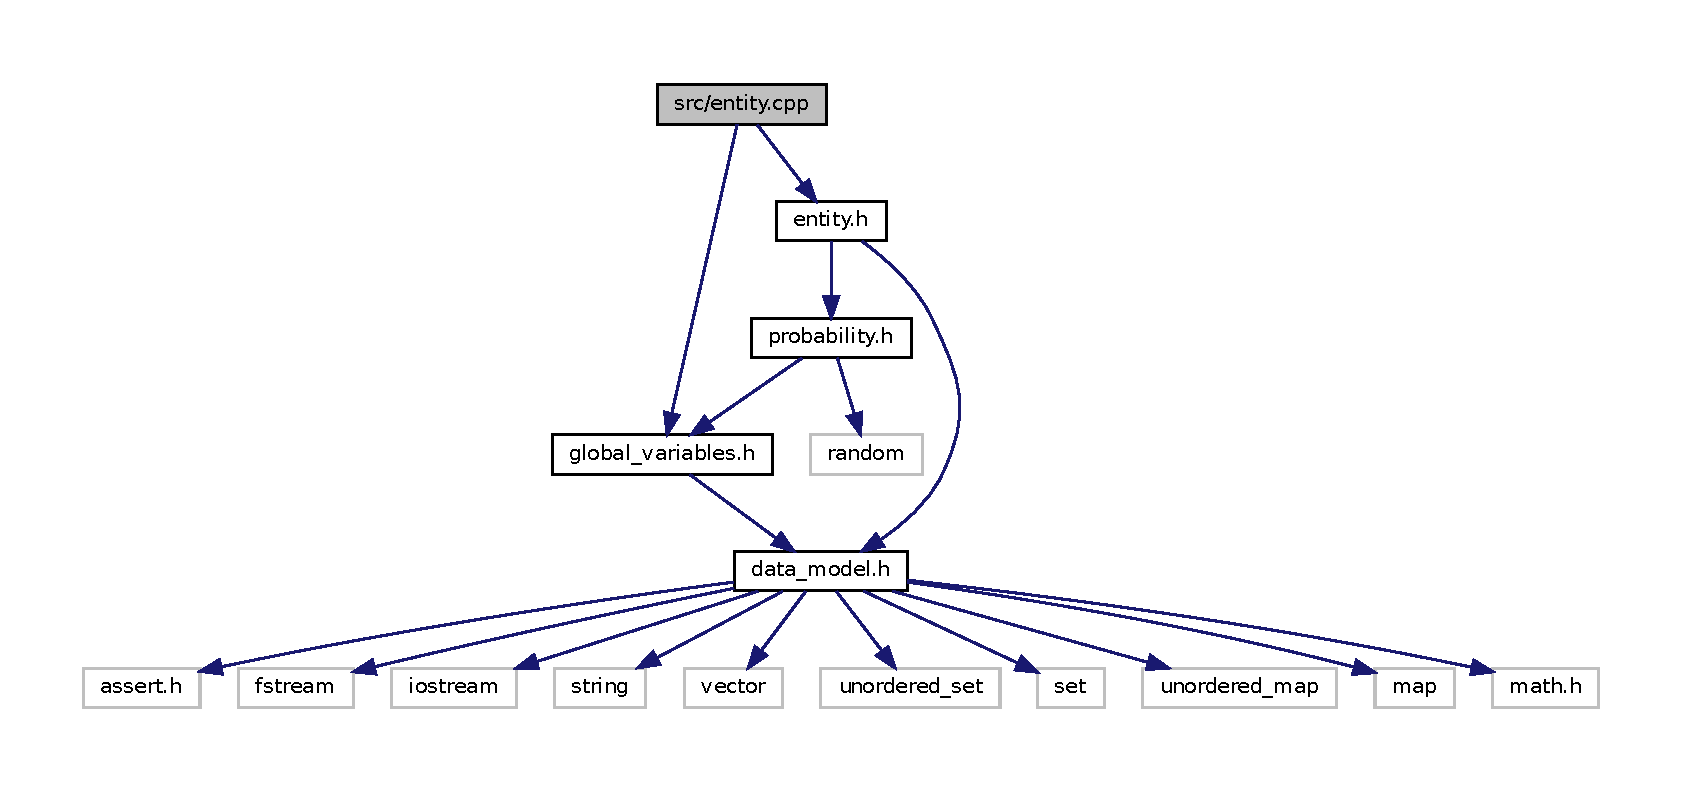
\includegraphics[width=350pt]{d8/d92/entity_8cpp__incl}
\end{center}
\end{figure}
\subsection*{Functions}
\begin{DoxyCompactItemize}
\item 
\hyperlink{namespacetricl_a57273122278e8b301844e2a2e1f0742f}{entity} \hyperlink{entity_8cpp_a0a2d9d57b1737f98889d96db80b44ea4}{add\+\_\+entity} (\hyperlink{namespacetricl_afd4de3aedd5e48cf955f03457386e98f}{entity\+\_\+type} et, string elabel)
\begin{DoxyCompactList}\small\item\em Add a new entity of a specific type. \end{DoxyCompactList}\item 
\hyperlink{namespacetricl_a57273122278e8b301844e2a2e1f0742f}{entity} \hyperlink{entity_8cpp_a98c686b5512ec703bd0da855cd296f24}{random\+\_\+entity} (\hyperlink{namespacetricl_afd4de3aedd5e48cf955f03457386e98f}{entity\+\_\+type} et)
\begin{DoxyCompactList}\small\item\em Return a random entity of a specific type. \end{DoxyCompactList}\end{DoxyCompactItemize}


\subsection{Detailed Description}
Handling of entities. 

\begin{DoxyAuthor}{Author}
Jobst Heitzig, Potsdam Institute for Climate Impact Research, \href{mailto:heitzig@pik-potsdam.de}{\tt heitzig@pik-\/potsdam.\+de} 
\end{DoxyAuthor}
\begin{DoxyDate}{Date}
Mar 30, 2020 
\end{DoxyDate}


\subsection{Function Documentation}
\mbox{\Hypertarget{entity_8cpp_a0a2d9d57b1737f98889d96db80b44ea4}\label{entity_8cpp_a0a2d9d57b1737f98889d96db80b44ea4}} 
\index{entity.\+cpp@{entity.\+cpp}!add\+\_\+entity@{add\+\_\+entity}}
\index{add\+\_\+entity@{add\+\_\+entity}!entity.\+cpp@{entity.\+cpp}}
\subsubsection{\texorpdfstring{add\+\_\+entity()}{add\_entity()}}
{\footnotesize\ttfamily \hyperlink{namespacetricl_a57273122278e8b301844e2a2e1f0742f}{entity} add\+\_\+entity (\begin{DoxyParamCaption}\item[{\hyperlink{namespacetricl_afd4de3aedd5e48cf955f03457386e98f}{entity\+\_\+type}}]{et,  }\item[{string}]{elabel }\end{DoxyParamCaption})}



Add a new entity of a specific type. 

(the entity is not returned) 
\begin{DoxyParams}[1]{Parameters}
\mbox{\tt in}  & {\em et} & entity type of the entity to be generated anew. \\
\hline
\mbox{\tt in}  & {\em elabel} & entity label (if \char`\"{}\char`\"{}, will be generated) \\
\hline
\end{DoxyParams}
\mbox{\Hypertarget{entity_8cpp_a98c686b5512ec703bd0da855cd296f24}\label{entity_8cpp_a98c686b5512ec703bd0da855cd296f24}} 
\index{entity.\+cpp@{entity.\+cpp}!random\+\_\+entity@{random\+\_\+entity}}
\index{random\+\_\+entity@{random\+\_\+entity}!entity.\+cpp@{entity.\+cpp}}
\subsubsection{\texorpdfstring{random\+\_\+entity()}{random\_entity()}}
{\footnotesize\ttfamily \hyperlink{namespacetricl_a57273122278e8b301844e2a2e1f0742f}{entity} random\+\_\+entity (\begin{DoxyParamCaption}\item[{\hyperlink{namespacetricl_afd4de3aedd5e48cf955f03457386e98f}{entity\+\_\+type}}]{et }\end{DoxyParamCaption})}



Return a random entity of a specific type. 

The entity is drawn uniformly at random. 
\begin{DoxyParams}[1]{Parameters}
\mbox{\tt in}  & {\em et} & Entity type of which a random entity is needed \\
\hline
\end{DoxyParams}

\hypertarget{event_8cpp}{}\section{src/event.cpp File Reference}
\label{event_8cpp}\index{src/event.\+cpp@{src/event.\+cpp}}


Handling of events.  


{\ttfamily \#include $<$assert.\+h$>$}\\*
{\ttfamily \#include $<$iostream$>$}\\*
{\ttfamily \#include \char`\"{}debugging.\+h\char`\"{}}\\*
{\ttfamily \#include \char`\"{}data\+\_\+model.\+h\char`\"{}}\\*
{\ttfamily \#include \char`\"{}global\+\_\+variables.\+h\char`\"{}}\\*
{\ttfamily \#include \char`\"{}entity.\+h\char`\"{}}\\*
{\ttfamily \#include \char`\"{}angle.\+h\char`\"{}}\\*
{\ttfamily \#include \char`\"{}link.\+h\char`\"{}}\\*
{\ttfamily \#include \char`\"{}probability.\+h\char`\"{}}\\*
{\ttfamily \#include \char`\"{}event.\+h\char`\"{}}\\*
{\ttfamily \#include \char`\"{}io.\+h\char`\"{}}\\*
Include dependency graph for event.\+cpp\+:
\nopagebreak
\begin{figure}[H]
\begin{center}
\leavevmode
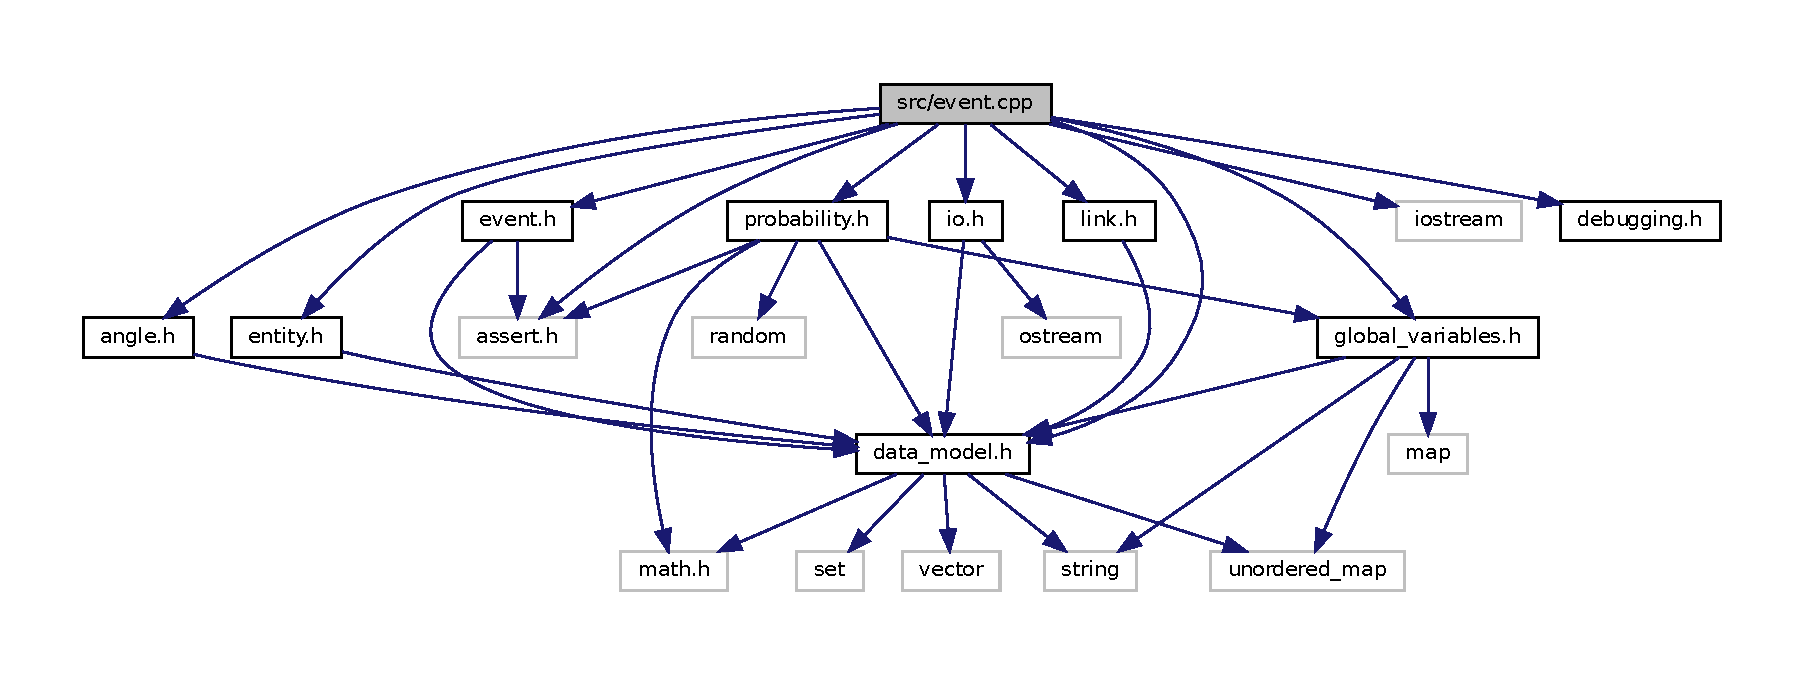
\includegraphics[width=350pt]{d6/d99/event_8cpp__incl}
\end{center}
\end{figure}
\subsection*{Macros}
\begin{DoxyCompactItemize}
\item 
\#define {\bfseries I\+F\+\_\+12}~if (which == 0)\hypertarget{event_8cpp_ac1e75a2e1d58d4f43aaa35324bb26538}{}\label{event_8cpp_ac1e75a2e1d58d4f43aaa35324bb26538}

\item 
\#define {\bfseries I\+F\+\_\+23}~if (which == 1)\hypertarget{event_8cpp_a0add313a6fd3d8fae54c55f125be6f0f}{}\label{event_8cpp_a0add313a6fd3d8fae54c55f125be6f0f}

\end{DoxyCompactItemize}
\subsection*{Functions}
\begin{DoxyCompactItemize}
\item 
bool \hyperlink{event_8cpp_ab8644632b851d99741826fb61fb703bd}{event\+\_\+is\+\_\+scheduled} (\hyperlink{structevent}{event} \&ev, \hyperlink{structevent__data}{event\+\_\+data} $\ast$evd\+\_\+)
\begin{DoxyCompactList}\small\item\em Return whether a future instance of the event is scheduled. \end{DoxyCompactList}\item 
void {\bfseries \+\_\+schedule\+\_\+event} (\hyperlink{structevent}{event} \&ev, \hyperlink{structevent__data}{event\+\_\+data} $\ast$evd\+\_\+, double left\+\_\+tail, double right\+\_\+tail)\hypertarget{event_8cpp_a4048cb830821ab767f91d751e7bd1f37}{}\label{event_8cpp_a4048cb830821ab767f91d751e7bd1f37}

\item 
void {\bfseries schedule\+\_\+event} (\hyperlink{structevent}{event} \&ev, \hyperlink{structevent__data}{event\+\_\+data} $\ast$evd\+\_\+, double left\+\_\+tail, double right\+\_\+tail)\hypertarget{event_8cpp_a269d75ea7ef6f98c60705a062e98f4e0}{}\label{event_8cpp_a269d75ea7ef6f98c60705a062e98f4e0}

\item 
void {\bfseries reschedule\+\_\+event} (\hyperlink{structevent}{event} \&ev, \hyperlink{structevent__data}{event\+\_\+data} $\ast$evd\+\_\+, double left\+\_\+tail, double right\+\_\+tail)\hypertarget{event_8cpp_ad37a5884bb4d210596ad150d6efafed0}{}\label{event_8cpp_ad37a5884bb4d210596ad150d6efafed0}

\item 
void {\bfseries add\+\_\+event} (\hyperlink{structevent}{event} \&ev)\hypertarget{event_8cpp_aef94fa11ff43b90a11586d18670f2700}{}\label{event_8cpp_aef94fa11ff43b90a11586d18670f2700}

\item 
void {\bfseries remove\+\_\+event} (\hyperlink{structevent}{event} \&ev, \hyperlink{structevent__data}{event\+\_\+data} $\ast$evd\+\_\+)\hypertarget{event_8cpp_a55e7ed06ea3900949b3bb7a464670054}{}\label{event_8cpp_a55e7ed06ea3900949b3bb7a464670054}

\item 
void {\bfseries conditionally\+\_\+remove\+\_\+event} (\hyperlink{structevent}{event} \&ev)\hypertarget{event_8cpp_a875f0862466ff1b831fee64602d92d76}{}\label{event_8cpp_a875f0862466ff1b831fee64602d92d76}

\item 
void {\bfseries update\+\_\+adjacent\+\_\+events} (\hyperlink{structevent}{event} \&ev)\hypertarget{event_8cpp_adc013b33a8b8afbb4f75c8c95dc3b93a}{}\label{event_8cpp_adc013b33a8b8afbb4f75c8c95dc3b93a}

\item 
void {\bfseries add\+\_\+reverse\+\_\+event} (\hyperlink{structevent}{event} \&old\+\_\+ev)\hypertarget{event_8cpp_aec4dd06c452378363b04a58a0cfe8f8b}{}\label{event_8cpp_aec4dd06c452378363b04a58a0cfe8f8b}

\item 
void {\bfseries perform\+\_\+event} (\hyperlink{structevent}{event} \&ev)\hypertarget{event_8cpp_af13ceffde477e67e6d9418750ce45107}{}\label{event_8cpp_af13ceffde477e67e6d9418750ce45107}

\item 
bool {\bfseries pop\+\_\+next\+\_\+event} ()\hypertarget{event_8cpp_ad57de4475b376dedfc003a1b09cfece8}{}\label{event_8cpp_ad57de4475b376dedfc003a1b09cfece8}

\end{DoxyCompactItemize}


\subsection{Detailed Description}
Handling of events. 

An event is a tuple \{ec, e1, rat13, e3\} where ec is the event class (E\+C\+\_\+\+E\+ST or E\+C\+\_\+\+T\+E\+RM for establishment or termination of a relationship, E\+C\+\_\+\+A\+CT for the occurrence of an act), e1 and e3 are the affected entities, and rat13 is the relationship or action type.

An event type is a tuple (ec, et1, rat13, et3\} where et1, et3 are two entity types.

An event\textquotesingle{}s variable data (current attempt rate, success probability units, and next scheduled timepoint) is stored in a separate struct of type \hyperlink{structevent__data}{event\+\_\+data}.

\begin{DoxyAuthor}{Author}
Jobst Heitzig, Potsdam Institute for Climate Impact Research, \href{mailto:heitzig@pik-potsdam.de}{\tt heitzig@pik-\/potsdam.\+de} 
\end{DoxyAuthor}
\begin{DoxyDate}{Date}
Mar 30, 2020 
\end{DoxyDate}


\subsection{Function Documentation}
\index{event.\+cpp@{event.\+cpp}!event\+\_\+is\+\_\+scheduled@{event\+\_\+is\+\_\+scheduled}}
\index{event\+\_\+is\+\_\+scheduled@{event\+\_\+is\+\_\+scheduled}!event.\+cpp@{event.\+cpp}}
\subsubsection[{\texorpdfstring{event\+\_\+is\+\_\+scheduled(event \&ev, event\+\_\+data $\ast$evd\+\_\+)}{event_is_scheduled(event &ev, event_data *evd_)}}]{\setlength{\rightskip}{0pt plus 5cm}bool event\+\_\+is\+\_\+scheduled (
\begin{DoxyParamCaption}
\item[{{\bf event} \&}]{ev, }
\item[{{\bf event\+\_\+data} $\ast$}]{evd\+\_\+}
\end{DoxyParamCaption}
)}\hypertarget{event_8cpp_ab8644632b851d99741826fb61fb703bd}{}\label{event_8cpp_ab8644632b851d99741826fb61fb703bd}


Return whether a future instance of the event is scheduled. 


\begin{DoxyParams}[1]{Parameters}
\mbox{\tt in}  & {\em ev} & the event to check, passed by reference for performance \\
\hline
\mbox{\tt in}  & {\em evd\+\_\+} & the corresponding variable event data, passed by pointer for performance \\
\hline
\end{DoxyParams}

\hypertarget{tricl_8cpp}{}\section{src/tricl.cpp File Reference}
\label{tricl_8cpp}\index{src/tricl.\+cpp@{src/tricl.\+cpp}}


Tri\+Cl, a generic model of social dynamics.  


{\ttfamily \#include $<$iostream$>$}\newline
{\ttfamily \#include \char`\"{}global\+\_\+variables.\+h\char`\"{}}\newline
{\ttfamily \#include \char`\"{}config.\+h\char`\"{}}\newline
{\ttfamily \#include \char`\"{}init.\+h\char`\"{}}\newline
{\ttfamily \#include \char`\"{}simulate.\+h\char`\"{}}\newline
{\ttfamily \#include \char`\"{}finish.\+h\char`\"{}}\newline
Include dependency graph for tricl.\+cpp\+:\nopagebreak
\begin{figure}[H]
\begin{center}
\leavevmode
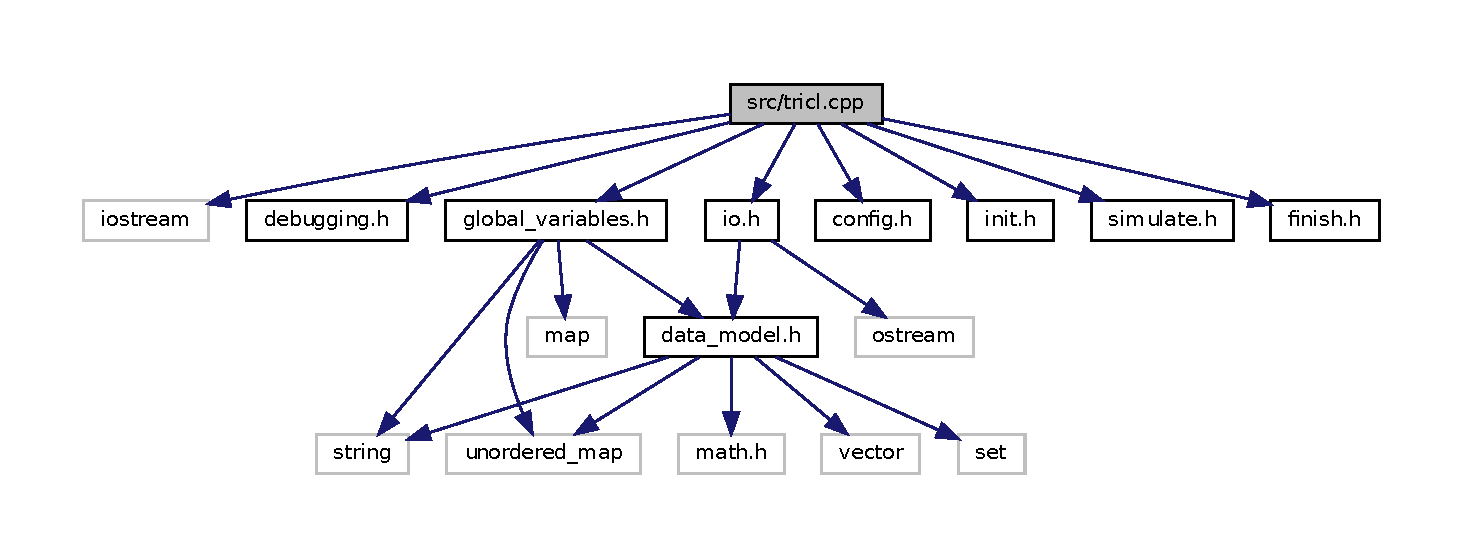
\includegraphics[width=350pt]{d0/d26/tricl_8cpp__incl}
\end{center}
\end{figure}
\subsection*{Functions}
\begin{DoxyCompactItemize}
\item 
\mbox{\Hypertarget{tricl_8cpp_ade42974a32e89c168c97127bbc971da4}\label{tricl_8cpp_ade42974a32e89c168c97127bbc971da4}} 
void \hyperlink{tricl_8cpp_ade42974a32e89c168c97127bbc971da4}{parse\+\_\+args} (int argc, const char $\ast$argv\mbox{[}$\,$\mbox{]})
\begin{DoxyCompactList}\small\item\em parse the command line arguments \end{DoxyCompactList}\item 
\mbox{\Hypertarget{tricl_8cpp_ac0f2228420376f4db7e1274f2b41667c}\label{tricl_8cpp_ac0f2228420376f4db7e1274f2b41667c}} 
int \hyperlink{tricl_8cpp_ac0f2228420376f4db7e1274f2b41667c}{main} (int argc, const char $\ast$argv\mbox{[}$\,$\mbox{]})
\begin{DoxyCompactList}\small\item\em main function of the tricl executable \end{DoxyCompactList}\end{DoxyCompactItemize}
\subsection*{Variables}
\begin{DoxyCompactItemize}
\item 
\mbox{\Hypertarget{tricl_8cpp_a6ff215d62218bc381c50ab2e7ef4731d}\label{tricl_8cpp_a6ff215d62218bc381c50ab2e7ef4731d}} 
string \hyperlink{tricl_8cpp_a6ff215d62218bc381c50ab2e7ef4731d}{config\+\_\+yaml\+\_\+filename}
\begin{DoxyCompactList}\small\item\em filename of configuration file \end{DoxyCompactList}\end{DoxyCompactItemize}


\subsection{Detailed Description}
Tri\+Cl, a generic model of social dynamics. 

\begin{DoxyAuthor}{Author}
Jobst Heitzig, Potsdam Institute for Climate Impact Research, \href{mailto:heitzig@pik-potsdam.de}{\tt heitzig@pik-\/potsdam.\+de} 
\end{DoxyAuthor}
\begin{DoxyDate}{Date}
Oct 18, 2019 
\end{DoxyDate}

%--- End generated contents ---

% Index
\backmatter
\newpage
\phantomsection
\clearemptydoublepage
\addcontentsline{toc}{chapter}{Index}
\printindex

\end{document}
